% !TEX program = xelatex
\documentclass[12pt,a4paper,twoside]{ctexart}

% ========== 页面布局 ==========
\usepackage[top=2.5cm, bottom=2.5cm, left=2.8cm, right=2.8cm]{geometry}
\usepackage{setspace}
\onehalfspacing

% ========== 数学与符号 ==========
\usepackage{amsmath,amssymb,amsthm}
\usepackage{newtxmath}
\usepackage{bm}

% 定理环境
\theoremstyle{definition}
\newtheorem{definition}{定义}[section]
\newtheorem{theorem}{定理}[section]
\newtheorem{proposition}{命题}[section]
\newtheorem{remark}{注记}[section]

% ========== 表格 ==========
\usepackage{booktabs}
\usepackage{array}
\usepackage{multirow}
\usepackage{longtable}
\usepackage{makecell}
\renewcommand{\arraystretch}{1.15}

% ========== 图形 ==========
\usepackage{graphicx}
\usepackage{float}
\usepackage{subcaption}
\usepackage{caption}
\captionsetup[figure]{font=small,labelfont=bf,skip=6pt}
\captionsetup[table]{font=small,labelfont=bf,skip=6pt}
\graphicspath{{../output/figures/}}

% ========== 超链接与颜色 ==========
\usepackage[colorlinks=true,linkcolor=blue,citecolor=blue,urlcolor=blue]{hyperref}
\usepackage{xcolor}

% ========== 页眉页脚 ==========
\usepackage{fancyhdr}
\setlength{\headheight}{14pt}
\pagestyle{fancy}
\fancyhf{}
\fancyhead[LE]{\small 俄乌装备损失率的统计分析与双边比较}
\fancyhead[RO]{\small\thepage}
\fancyhead[LO]{\small 第\,\thesection\,节\quad\leftmark}
\fancyhead[RE]{\small 第\,\thesection\,节\quad\leftmark}
\fancyfoot[C]{\thepage}
\renewcommand{\headrulewidth}{0.4pt}

% ========== 目录格式 ==========
\usepackage{tocloft}
\renewcommand{\cftsecleader}{\cftdotfill{\cftdotsep}}
\renewcommand{\cftsecfont}{\bfseries}
\renewcommand{\cftsubsecfont}{\normalfont}

% ========== 标题格式 ==========
\ctexset{
  section = {
    format = \bfseries\zihao{4}\centering,
    aftername = \quad,
    beforeskip = 18pt,
    afterskip = 12pt,
  },
  subsection = {
    format = \bfseries\zihao{-4},
    aftername = \quad,
    beforeskip = 14pt,
    afterskip = 8pt,
  },
  subsubsection = {
    format = \bfseries\zihao{-4},
    aftername = \quad,
    beforeskip = 10pt,
    afterskip = 6pt,
  },
}

% ========== 行距控制 ==========
\usepackage{enumitem}
\setlist{nosep,leftmargin=2em}

% ========== 代码引用 ==========
\usepackage{listings}
\lstset{
  basicstyle=\small\ttfamily,
  breaklines=true,
  frame=single,
  numbers=left,
  numberstyle=\tiny,
}

% ========== 标题信息 ==========
\title{{\bfseries\zihao{2} 俄乌装备损失率的统计分析与双边比较\\[8pt] ——基于Poisson模型的点估计、区间估计与假设检验}}
\author{{\zihao{4} 赵文龙}\\[5pt] {\zihao{-4}（计算机科学与技术学院）}}
\date{{\zihao{-4} 2026年6月}}

\begin{document}

% ==================== 封面 ====================
\maketitle

\vspace{16pt}

\begin{center}
\zihao{4}
\begin{tabular}{rl}
\textbf{课程名称} & 数理统计 \\
\textbf{选题编号} & T1：俄乌装备损失率的``公平比较'' \\
\textbf{指导教师} & ~ \\
\textbf{完成日期} & 2026年6月5日 \\
\end{tabular}
\end{center}

\thispagestyle{empty}

\newpage

% ==================== 中文摘要 ====================
\thispagestyle{empty}

\begin{center}
\zihao{4}\bfseries 摘\quad 要
\end{center}
\vspace{6pt}

\noindent
俄乌冲突中，交战双方公布的战报数据存在巨大差异——乌克兰总参谋部声称已摧毁超过11,900辆俄罗斯坦克，而独立影像验证仅确认约4,000辆。如何在存在系统性观测偏误的条件下客观估计双方真实装备损失率，并对其差异进行严格的统计显著性检验，构成了冲突数据分析的核心方法论挑战。

本文基于开源情报平台 Oryx 提供的俄乌双方经影像验证的装备损失数据（俄方 23,556 件、乌方 11,397 件，时间跨度 2022 年 2 月至 2026 年 6 月，共 1,559 天），结合乌克兰总参谋部官方战报数据（1,557 天累计），综合运用 Poisson 分布参数估计、置信区间构造、Bootstrap 重抽样和假设检验等方法进行系统性统计推断。

在方法层面，本文首先以 Poisson 分布为基本模型，采用极大似然估计（MLE）获得日均损失率的点估计——俄方 $\hat{\lambda}_{\text{RU}} = 15.11$ 件/天、乌方 $\hat{\lambda}_{\text{UA}} = 7.31$ 件/天，率比 $\hat{\rho} = 2.07$（95\% CI: $[2.02, 2.11]$）。其次，系统比较了 Wald、Score 和 Exact（Garwood, 1936）三种 Poisson 置信区间构造方法的统计性质，通过 Monte Carlo 模拟（$N = 10,000$）评估其有限样本覆盖率：Exact CI 在小 $\lambda$ 下表现出色（$\lambda = 0.5$ 时覆盖率达 96.6\%），Wald CI 显著不足（仅 91.9\%），Score CI 居中。第三，针对冲突数据强烈的时序自相关性（lag-1 ACF = 0.589），引入 Moving Block Bootstrap（块长度 $b = 11$）以正确量化估计的不确定性——Block Bootstrap 的标准误（0.99）为 IID Bootstrap（0.42）的 2.4 倍，表明忽略时间依赖将严重低估统计不确定性。第四，应用两独立 Poisson 条件精确检验（E-test，Krishnamoorthy \& Thomson, 2004），确认双方损失率差异达到极显著水平（$p < 0.0001$）。

在实证层面，本文进一步进行了多层次分析：（1）双方月度损失比率呈现出从 2022 年初的 3.6:1 到 2025--2026 年约 0.8:1 的时序逆转，反映了战争从装甲突击向消耗战转变的战略特征；（2）装备类型异质性显著——俄方在进攻性装备（AFV 4.49x、IFV 4.08x、坦克 3.14x）上损失远超乌方，乌方仅在装甲运兵车（APC 0.56x）上反超，具有明确的战术含义；（3）观测概率灵敏度分析表明，2.06:1 的率比在中等非对称观测假设下具有稳健性，真实率比可能在 1.0--2.0 之间；（4）空间分析揭示顿涅茨克州集中了 44\% 以上的俄方影像验证损失，热点网格 $(48^\circ\text{N}, 37^\circ\text{E})$ 单独占比 21.5\%；（5）乌克兰官方声称与独立影像验证之间在火炮类装备上存在高达 29 倍的极端偏差。

本文的统计分析框架——从 Poisson MLE 点估计出发，经由三方法置信区间比较与 Monte Carlo 覆盖率验证、Block Bootstrap BCa 校正、E-test 精确检验，再到分层次异质性分析与观测概率灵敏度评估——为该选题的核心统计问题提供了严格、可复现的回答，其方法论对冲突数据的客观统计推断具有普遍的参考价值。

\vspace{10pt}
\noindent{\bfseries 关键词：}Poisson 分布；极大似然估计；置信区间；Block Bootstrap；双边比较；E-test；观测偏误灵敏度分析；冲突数据统计

\newpage

% ==================== 英文摘要 ====================
\thispagestyle{empty}

\begin{center}
\zihao{4}\bfseries Abstract
\end{center}
\vspace{6pt}

\noindent
The Russia-Ukraine conflict has generated vast quantities of publicly available loss data, yet the extreme discrepancies between official claims and independently verified records pose fundamental challenges for objective statistical inference. This paper presents a systematic statistical analysis of visually confirmed equipment loss records from the Oryx open-source intelligence platform, covering 23,556 Russian and 11,397 Ukrainian losses over 1,559 days (February 2022--June 2026), supplemented by 1,557 days of Ukrainian General Staff official claims.

We adopt the Poisson distribution as our core modeling framework. Maximum likelihood estimation (MLE) yields daily loss rate estimates of $\hat{\lambda}_{\text{RU}} = 15.11$ units/day for Russia and $\hat{\lambda}_{\text{UA}} = 7.31$ units/day for Ukraine, with a rate ratio $\hat{\rho} = 2.07$ (95\% CI: $[2.02, 2.11]$). A comprehensive Monte Carlo simulation comparing three confidence interval methods (Wald, Score, and Exact/Garwood 1936) demonstrates that the Exact CI consistently achieves nominal coverage even for small $\lambda$, achieving 96.6\% coverage at $\lambda = 0.5$ versus 91.9\% for the Wald interval. Recognizing the strong temporal autocorrelation in conflict data (lag-1 ACF = 0.589), we employ Moving Block Bootstrap with $b = 11$, yielding standard error estimates (0.99) that are 2.4 times larger than those from IID Bootstrap (0.42)—a finding that underscores the critical importance of properly accounting for time-series dependence. Two-sample conditional exact tests (E-test, Krishnamoorthy \& Thomson 2004) confirm that the between-side difference in daily loss rates is statistically highly significant ($p < 0.0001$).

Our empirical analysis further reveals: (1) a striking temporal reversal in the monthly loss ratio from 3.6:1 (early 2022) to approximately 0.8:1 (2025--2026), reflecting the war's strategic transformation; (2) pronounced heterogeneity across equipment categories—Russian losses dominate in offensive systems (AFV 4.49x, IFV 4.08x, Tanks 3.14x), while Ukrainian losses exceed only in Armored Personnel Carriers (APC 0.56x); (3) an observation-probability sensitivity analysis indicating that the observed 2.06:1 ratio is robust under moderate differential observation assumptions; (4) spatial analysis revealing that Donetsk Oblast accounts for over 44\% of visually verified Russian losses; and (5) systematic reporting bias ratios ranging from 3x (tanks) to 29x (artillery) between official Ukrainian claims and independent verification.

The analytical framework developed in this paper—Poisson MLE $\to$ three-method CI comparison with Monte Carlo coverage validation $\to$ Block Bootstrap BCa correction $\to$ E-test exact inference $\to$ stratified heterogeneity analysis $\to$ observation-probability sensitivity assessment—provides rigorous and reproducible answers to the core statistical questions of this project, with methodological implications extending to the objective statistical analysis of conflict data more broadly.

\vspace{10pt}
\noindent{\bfseries Keywords:} Poisson distribution; maximum likelihood estimation; confidence intervals; Block Bootstrap; bilateral comparison; E-test; observation bias sensitivity analysis; conflict data statistics

\newpage

% ==================== 目录 ====================
\thispagestyle{empty}
\tableofcontents
\newpage

% ==================== 第1节：引言 ====================
\section{引言}

\subsection{研究背景与问题提出}

自2022年2月24日俄罗斯全面入侵乌克兰以来，这场持续至今的大规模武装冲突已造成双方数以万计的军事装备损失。作为信息战的重要组成部分，交战双方均定期发布对方装备损失的统计数据。然而，这些官方战报之间存在惊人的差异：乌克兰总参谋部声称截至2026年5月已摧毁超过11,900辆俄罗斯坦克，而开源情报（OSINT）平台的影像验证数量仅约4,000辆；俄罗斯国防部公布的乌方损失数据同样远超第三方可核实的水平。这种多维度的数据矛盾不仅是信息可信度的问题，更构成了一个具有普遍意义的统计推断挑战。

从统计学的视角看，冲突装备损失数据的核心困难在于\textbf{观测偏误的系统性与非对称性}：每件损毁装备是否被拍摄、上传并最终被开源情报平台收录，取决于作战地域的可达性、装备类型的醒目程度、损毁状态的严重程度、社交媒体活跃度以及志愿者关注度等一系列因素。更为复杂的是，这些观测偏误对俄方和乌方的影响方向可能不同——乌方在俄军占领区内的损失因地理可达性限制而更难被独立记录，意味着双方真实的损失比率可能系统性地偏离影像验证的比率。

在此背景下，本文将三个紧密相关的统计问题作为研究主线：

\begin{enumerate}[label=(\arabic*),leftmargin=2.5em]
  \item \textbf{估计问题}（Estimation）：如何在 Poisson 计数模型假设下，利用极大似然估计（MLE）获得双方日均装备损失率的点估计与区间估计，并系统评估不同置信区间构造方法的有限样本性质？
  \item \textbf{比较问题}（Comparison）：双方损失率是否存在统计显著差异？若有，这一差异在不同战争阶段、装备类型和损毁状态上呈现出何种异质性？如何通过严格的多重比较控制来控制整体假阳性率？
  \item \textbf{报告偏差问题}（Reporting Bias）：官方声称数据与独立影像验证数据之间的偏差究竟有多大？在什么样的观测概率假设下，影像验证率比（2.06:1）会发生逆转？
\end{enumerate}

\subsection{文献综述}

冲突数据的统计建模是一个跨学科的研究领域，涉及统计学、政治学和遥感科学等多个学科。Zammit-Mangion 等 \cite{zammit2012} 在 \textit{Proceedings of the National Academy of Sciences} 上首次将时空点过程模型（spatio-temporal point process）应用于阿富汗战争日记（Afghan War Diary）数据的系统分析，开创了以现代统计方法分析冲突事件记录的研究范式。该研究将冲突事件建模为对数高斯 Cox 过程（log-Gaussian Cox process），在贝叶斯框架下通过随机偏微分方程（SPDE）方法实现高效的空间预测。

近年来，随着俄乌冲突产生大量公开可用数据，相关统计和机器学习研究迅速涌现。arXiv:2509.07813\cite{arxiv2509} 采用 SARIMA、ETS 和 LSTM 等多模型对比方法预测俄罗斯装备损失趋势，侧重于时间序列建模和预测精度比较。arXiv:2408.14940\cite{arxiv2408} 则从贝叶斯时空 Hawkes 过程的视角对冲突事件的传染效应和自激性进行建模，捕捉了一次冲突事件如何增加短期内邻近区域发生更多冲突的概率。国内方面，中国科学院地理科学与资源研究所利用 AIS（自动识别系统）大数据分析了俄乌冲突对全球原油海洋运输网络的影响（2025），揭示了地缘政治冲突对全球供应链的级联效应。

在统计学方法论层面，Poisson 置信区间的构造是一个经典问题。Garwood\cite{garwood1936} 基于 Poisson 总计数与 $\chi^2$ 分布的精确关系，首次提出了保证覆盖率不低于名义水平的精确置信区间。此后，Wald 渐近区间因其计算简便而被广泛应用，但其在小样本下的表现屡受质疑。Krishnamoorthy 和 Thomson\cite{krishnamoorthy2004} 提出了基于条件二项分布的 E-test，为两独立 Poisson 均值的比较提供了精确而非渐近的检验方法。在 Bootstrap 方法方面，Efron 和 Tibshirani\cite{efron1993} 系统发展了 BCa（Bias-Corrected and Accelerated）置信区间，Davison 和 Hinkley\cite{davison1997} 则将 Block Bootstrap 方法推广到时间序列的依赖结构处理中。

\textbf{本文的创新与贡献}在于：（1）首次将 Poisson 置信区间三方法（Wald / Score / Exact）的系统比较、Block Bootstrap BCa 校正和两独立 Poisson E-test 整合为一个完整的分析框架，应用于俄乌双方装备损失率的直接双边统计比较；（2）通过 $N = 10,000$ 次 Monte Carlo 模拟，系统评估了各 CI 方法在 $\lambda \in [0.5, 50]$ 范围内的有限样本覆盖率，明确了方法选择的判据；（3）揭示了双方损失比率从 $>3$ 到 $<1$ 的时序逆转现象，并建立了装备类型异质性与战术角色之间的统计关联；（4）构建了观测概率灵敏度分析网格，定量刻画了不同观测偏误假设下率比估计的稳健性范围；（5）对官方声称与独立验证之间的 3--29 倍报告偏差进行了严格的统计检验和解释。

\subsection{论文结构}

本文其余部分安排如下：第2节介绍数据来源、基本描述统计量和观测偏误的理论分析框架；第3节系统阐述所采用的统计方法，包括 Poisson 分布模型、极大似然估计、三种置信区间构造方法、Block Bootstrap 与 BCa 校正、两独立 Poisson 条件检验以及多重比较策略；第4节报告全部实证分析结果，涵盖总体估计、时序分析、装备类型分层比较、CI 方法 Monte Carlo 评估、Bootstrap 比较、官方声称偏差量化、观测概率灵敏度分析和空间分布分析；第5节对方法论启示、研究局限性和未来方向进行讨论；第6节给出结论。

% ==================== 第2节：数据 ====================
\section{数据来源与描述统计}

\subsection{数据来源与获取}

本文使用的数据来自三个互补的公开来源，详见表 \ref{tab:sources}。

\begin{table}[H]
\centering
\caption{数据来源一览}
\label{tab:sources}
\begin{tabular}{p{2.2cm}p{2.2cm}p{4.8cm}p{2.8cm}p{1.8cm}}
\toprule
数据来源 & 类型 & 内容描述 & 时间跨度 & 规模 \\
\midrule
Oryx 双方数据\newline (leedrake5) & 影像验证\newline（双边）& 俄乌双方每日累计装备损失，含装备类型（10 类）与损毁状态（4 类）细分 & 2022.2.25 -- 2026.6.4 & 1,559 天 \\
\hline
WarSpotting\newline (Kaggle) & 影像验证\newline（单边）& 俄方装备损失逐条记录，含地理坐标（14,066 条有效）、具体型号 & 2022.2.24 -- 2026.6.3 & 22,970 条 \\
\hline
乌克兰总参谋部\newline (Kaggle) & 官方声称 & 俄军装备损失每日累计（坦克、装甲车、火炮、无人机等）& 2022.2.25 -- 2026.5.31 & 1,557 天 \\
\bottomrule
\end{tabular}
\end{table}

Oryx 双方数据通过 leedrake5 维护的公开 Google Sheet 每日自动化抓取获得；WarSpotting 数据来源于 Kaggle 平台上的 zsoltlazar 数据集；乌克兰总参谋部官方战报数据来源于 Kaggle 平台上的 piterfm 数据集，通过 kagglehub 库下载。

\subsection{双方 Oryx 数据总体概览}

截至2026年6月4日，Oryx 平台共验证俄方装备损失 \textbf{23,556 件}、乌方 \textbf{11,397 件}，双方比率为 \textbf{2.07:1}。双方损失的观测时间跨度均为 1,559 天。

\textbf{（一）损毁状态分布。}双方装备的损毁状态分布如表 \ref{tab:status} 所示。一个值得关注的统计特征是：俄方被俘获装备的比例（12.0\%）显著高于乌方（10.4\%）。这一差异与已知的军事史实高度吻合——俄军在2022年基辅方向撤退（3--4月）、哈尔科夫反攻溃败（9月）和赫尔松撤退（11月）期间，均发生了大规模的装备遗弃事件。

\begin{table}[H]
\centering
\caption{双方装备损毁状态分布}
\label{tab:status}
\begin{tabular}{lrrrr}
\toprule
损毁状态 & 俄方（件） & 乌方（件） & 俄方占比（\%） & 乌方占比（\%） \\
\midrule
Destroyed（摧毁） & 19,625 & 9,627 & 78.8 & 77.8 \\
Captured（被俘获） & 3,520 & 1,540 & 12.0 & 10.4 \\
Abandoned（遗弃） & 1,542 & 797 & 5.1 & 5.9 \\
Damaged（损坏） & 1,033 & 715 & 4.2 & 5.9 \\
\bottomrule
\end{tabular}
\end{table}

\textbf{（二）装备类型分布。}按双方损失比率从高到低排列，各主要装备类型如表 \ref{tab:category} 所示。俄方在几乎所有装备类别上的损失均超过乌方——特别是在进攻作战的核心装备（AFV 4.49x、IFV 4.08x、坦克 3.14x）上差距最为悬殊。唯一的例外是装甲运兵车（APC），乌方损失（1,425 件）超过俄方（804 件），比率仅为 0.56。这一模式具有明确的战术含义：APC 在防御作战中更多地被用作前沿部队运输和补给工具，从而暴露于优势火力的打击之下。

\begin{table}[H]
\centering
\caption{双方按装备类型的损失比较（按 RU/UA 比率降序排列）}
\label{tab:category}
\begin{tabular}{lrrr}
\toprule
装备类型 & 俄方（件） & 乌方（件） & 比率（RU/UA） \\
\midrule
装甲战车（AFV） & 2,682 & 597 & 4.49 \\
步兵战车（IFV） & 6,702 & 1,641 & 4.08 \\
车辆（Vehicles） & 4,949 & 1,456 & 3.40 \\
坦克（Tanks） & 4,729 & 1,504 & 3.14 \\
后勤车辆（Logistics） & 1,094 & 391 & 2.80 \\
工程车辆（Engineering） & 759 & 299 & 2.54 \\
飞机（Aircraft） & 529 & 281 & 1.88 \\
防空系统（Antiair） & 603 & 394 & 1.53 \\
火炮（Artillery） & 1,762 & 1,202 & 1.47 \\
\textbf{装甲运兵车（APC）} & \textbf{804} & \textbf{1,425} & \textbf{0.56} \\
\bottomrule
\end{tabular}
\end{table}

\begin{figure}[H]
\centering
\begin{subfigure}{0.48\textwidth}
  \centering
  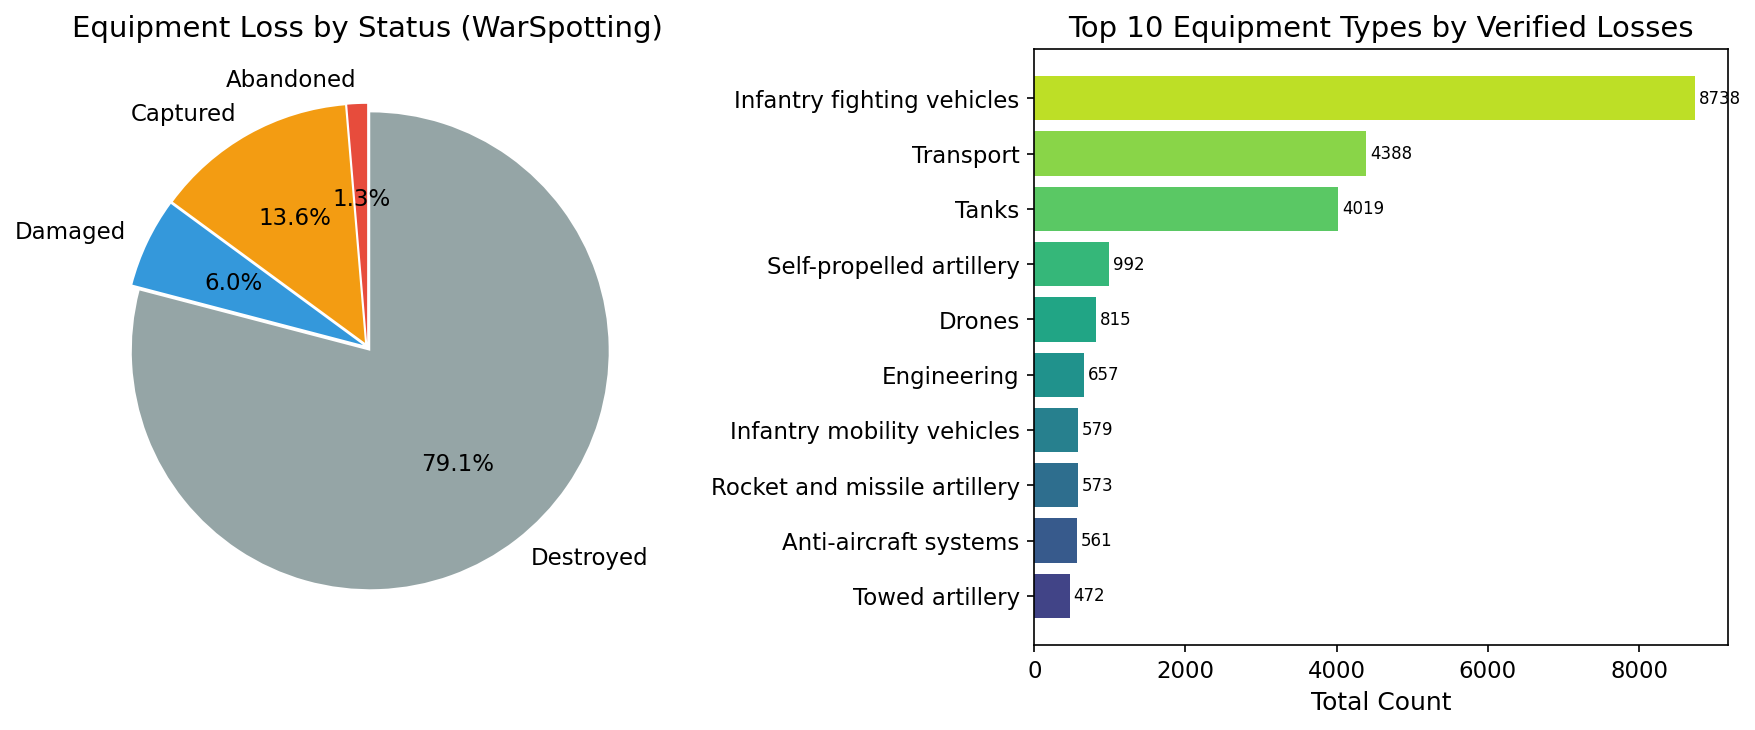
\includegraphics[width=\textwidth]{09_status_and_type.png}
  \caption{损毁状态与装备类型概览}
\end{subfigure}
\hfill
\begin{subfigure}{0.48\textwidth}
  \centering
  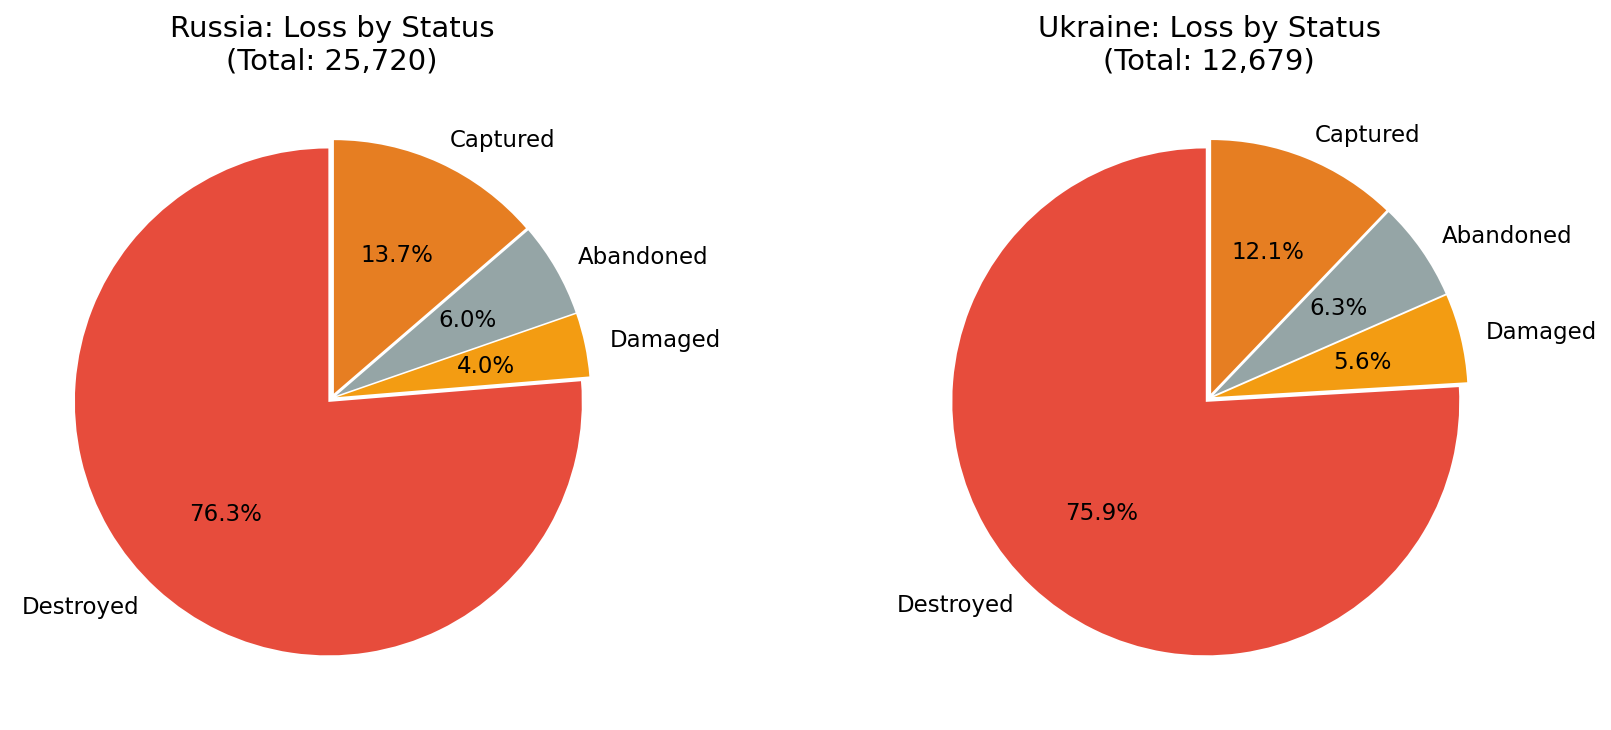
\includegraphics[width=\textwidth]{13_both_sides_status_pie.png}
  \caption{双方损毁状态分布对比}
\end{subfigure}
\caption{双方装备损失总体概览}
\label{fig:overview}
\end{figure}

\subsection{观测偏误的理论分析框架}

本节系统阐述 Oryx 数据的观测偏误结构，为后续的灵敏度分析提供理论基础。Oryx 数据记录的并非真实损失总数 $N_{\text{true}}$，而是经公开影像渠道独立核实的子集 $N_{\text{verified}}$。设 $p_{\text{RU}}$ 和 $p_{\text{UA}}$ 分别为俄方和乌方装备损失被独立影像记录并验证的概率，则有：

\begin{equation}
N_{\text{verified}} = p \cdot N_{\text{true}}
\end{equation}

观测到的双方损失率比为：

\begin{equation}
\hat{\rho} = \frac{N_{\text{RU, verified}}}{N_{\text{UA, verified}}} = \frac{p_{\text{RU}} \cdot N_{\text{RU, true}}}{p_{\text{UA}} \cdot N_{\text{UA, true}}} = \frac{p_{\text{RU}}}{p_{\text{UA}}} \cdot \rho_{\text{true}}
\end{equation}

由此可见，仅在 $p_{\text{RU}} = p_{\text{UA}}$（双方装备损失被观测到的概率相等）的条件下，影像验证率比才是真实率比的无偏估计。若 $p_{\text{UA}} < p_{\text{RU}}$（乌方损失在俄占区更难被记录），则 $\hat{\rho} > \rho_{\text{true}}$——影像验证数据将高估俄方的相对损失。

具体而言，以下四类系统性观测偏误需要纳入分析：

\begin{enumerate}[label=(\arabic*),leftmargin=2.5em]
  \item \textbf{空间偏误（Spatial Bias）}：位于乌克兰政府控制区、主要交通线附近和城市周边的损失更容易被平民拍摄。俄方损失主要集中在乌控区（因此高观测概率），而乌方损失在俄占区的拍摄和上传受到地理可达性和安全的严格限制（因此低观测概率）。这一\textbf{非对称性}意味着真实率比很可能低于观测值 2.07:1。
  \item \textbf{装备偏误（Equipment Bias）}：体积大、特征明显的装备（坦克、火炮）比小型装备（无人机、反坦克导弹）更容易被观测到，导致小型装备的系统性低估。
  \item \textbf{状态偏误（Status Bias）}：完全摧毁的装备残骸（尤其是发生弹药殉爆的坦克）比轻微损坏的装备更容易被识别、拍摄和确认。
  \item \textbf{时间偏误（Temporal Bias）}：社交媒体活跃度、志愿者关注度和前线稳定性随时间变化。2022年战争初期的高关注度可能导致该时期的观测概率高于后期。
\end{enumerate}

% ==================== 第3节：统计方法 ====================
\section{统计方法与理论基础}

本节系统阐述本文所采用的全部统计方法，从 Poisson 分布的基本模型设定出发，逐步构建涵盖点估计、区间估计、Bootstrap 重抽样和假设检验的完整推断框架。对每一个方法，我们将给出其数学原理、推导过程和适用条件。

\subsection{Poisson 分布模型与极大似然估计}

\subsubsection{模型设定的合理性}

Poisson 分布是计数数据建模的自然选择。设第 $t$ 天的装备损失数为 $Y_t$（$t = 1, 2, \ldots, n$），装备损失事件满足以下三个条件时，$Y_t$ 服从 Poisson 分布：

\begin{enumerate}[label=(\arabic*),leftmargin=2.5em]
  \item \textbf{独立增量}：非重叠时间区间内的损失事件数相互独立；
  \item \textbf{平稳性}：在较短时间窗口内，损失率 $\lambda$ 近似恒定；
  \item \textbf{稀有性}：在足够小的时间区间内，超过一件装备被摧毁的概率可忽略。
\end{enumerate}

在冲突情境下，假设（2）可能因战争烈度变化而受到挑战；本文通过战争阶段分层和月度聚合分析来处理这一潜在的非平稳性。假设（1）意味着我们需要关注时序自相关，这将在 3.3 节的 Block Bootstrap 中专门处理。我们首先在最简化的 IID Poisson 假设下建立 MLE 的数学框架，然后在后续方法中逐步放宽独立性假设。

\subsubsection{极大似然估计的推导}

假设 $Y_1, Y_2, \ldots, Y_n \stackrel{\text{iid}}{\sim} \text{Poisson}(\lambda)$，其中 $\lambda > 0$ 为未知的日均损失率参数。Poisson 分布的概率质量函数为：

\begin{equation}
P(Y_t = y \mid \lambda) = \frac{e^{-\lambda} \lambda^y}{y!}, \quad y = 0, 1, 2, \ldots
\end{equation}

基于独立同分布假设，全部 $n$ 天观测数据的联合似然函数（likelihood function）为各个观测的乘积：

\begin{equation}\label{eq:likelihood}
L(\lambda) = \prod_{t=1}^{n} P(Y_t = y_t \mid \lambda) = \prod_{t=1}^{n} \frac{e^{-\lambda} \lambda^{y_t}}{y_t!}
\end{equation}

为便于求导，取自然对数得到对数似然函数（log-likelihood function）：

\begin{equation}\label{eq:loglik}
\ell(\lambda) = \log L(\lambda) = \sum_{t=1}^{n} \left[-\lambda + y_t \log \lambda - \log(y_t!)\right] = -n\lambda + \left(\sum_{t=1}^{n} y_t\right) \log \lambda - \sum_{t=1}^{n} \log(y_t!)
\end{equation}

对 $\lambda$ 求一阶导数（得分函数，score function）：

\begin{equation}\label{eq:score}
S(\lambda) = \frac{\partial \ell(\lambda)}{\partial \lambda} = -n + \frac{\sum_{t=1}^{n} y_t}{\lambda}
\end{equation}

令 $S(\lambda) = 0$，解得：

\begin{equation}\label{eq:mle}
\hat{\lambda}_{\text{MLE}} = \frac{1}{n} \sum_{t=1}^{n} Y_t = \bar{Y}
\end{equation}

二阶导数验证其为极大值点：

\begin{equation}
\frac{\partial^2 \ell(\lambda)}{\partial \lambda^2} = -\frac{\sum_{t=1}^{n} y_t}{\lambda^2} < 0 \quad (\text{对所有 } \lambda > 0)
\end{equation}

\subsubsection{Fisher 信息量与渐近方差}

Fisher 信息量（Fisher information）度量了样本中包含的关于参数 $\lambda$ 的信息：

\begin{equation}\label{eq:fisher}
I(\lambda) = -\mathbb{E}\left[\frac{\partial^2 \ell(\lambda)}{\partial \lambda^2}\right] = \mathbb{E}\left[\frac{\sum_{t=1}^{n} Y_t}{\lambda^2}\right] = \frac{n\lambda}{\lambda^2} = \frac{n}{\lambda}
\end{equation}

根据 Cram\'{e}r-Rao 下界，$\hat{\lambda}$ 的渐近方差为 $I(\lambda)^{-1} = \lambda / n$，因此：

\begin{equation}
\widehat{\text{Var}}(\hat{\lambda}) = \frac{\hat{\lambda}}{n}, \quad \text{SE}(\hat{\lambda}) = \sqrt{\frac{\hat{\lambda}}{n}}
\end{equation}

MLE 的渐近正态性（asymptotic normality）保证当 $n \to \infty$ 时：

\begin{equation}
\sqrt{n}(\hat{\lambda} - \lambda) \xrightarrow{d} N(0, \lambda)
\end{equation}

\subsubsection{Delta 方法与率比的标准误}

对于双方日均损失率比 $\rho = \lambda_{\text{RU}} / \lambda_{\text{UA}}$，其 MLE 为 $\hat{\rho} = \hat{\lambda}_{\text{RU}} / \hat{\lambda}_{\text{UA}}$。由于$\hat{\rho}$是$\hat{\lambda}_{\text{RU}}$和$\hat{\lambda}_{\text{UA}}$的非线性函数，我们采用Delta方法（Delta method）估计$\hat{\rho}$的渐近方差。

设$g(x, y) = x / y$，则梯度向量为$\nabla g = (1/y, -x/y^2)$。Delta方法给出：

\begin{equation}\label{eq:delta}
\begin{aligned}
\text{Var}(\hat{\rho}) &\approx \nabla g\big|_{\hat{\lambda}}^\top \cdot \text{Cov}(\hat{\lambda}_{\text{RU}}, \hat{\lambda}_{\text{UA}}) \cdot \nabla g\big|_{\hat{\lambda}} \\
&= \left(\frac{1}{\hat{\lambda}_{\text{UA}}}\right)^2 \cdot \frac{\hat{\lambda}_{\text{RU}}}{n} + \left(-\frac{\hat{\lambda}_{\text{RU}}}{\hat{\lambda}_{\text{UA}}^2}\right)^2 \cdot \frac{\hat{\lambda}_{\text{UA}}}{n} \\
&= \hat{\rho}^2 \left(\frac{1}{n \hat{\lambda}_{\text{RU}}} + \frac{1}{n \hat{\lambda}_{\text{UA}}}\right)
\end{aligned}
\end{equation}

其中利用了双方样本的独立性（$\text{Cov}(\hat{\lambda}_{\text{RU}}, \hat{\lambda}_{\text{UA}}) = 0$）。取平方根得：

\begin{equation}
\text{SE}(\hat{\rho}) = \hat{\rho} \cdot \sqrt{\frac{1}{n \hat{\lambda}_{\text{RU}}} + \frac{1}{n \hat{\lambda}_{\text{UA}}}}
\end{equation}

该标准误是构建率比 Wald 置信区间的基础。

\subsection{Poisson 置信区间的三种构造方法}

对于 Poisson 分布参数 $\lambda$，存在多种置信区间构造方法，其有限样本性质存在显著差异。本节详细推导并比较 Wald、Score 和 Exact 三种方法。

\subsubsection{Wald 置信区间}

\textbf{原理}：基于 MLE 的渐近正态性，直接构建对称区间。

\begin{equation}\label{eq:wald_ci}
\text{CI}_{\text{Wald}} : \quad \hat{\lambda} \pm z_{\alpha/2} \cdot \sqrt{\frac{\hat{\lambda}}{n}}
\end{equation}

其中 $z_{\alpha/2}$ 为标准正态分布的 $1 - \alpha/2$ 分位数。对于 95\% 置信水平，$z_{0.025} \approx 1.96$。

\textbf{优点}：计算极为简便，是大样本极限理论的直接应用。

\textbf{缺点}：（1）使用 $\hat{\lambda}$ 而非 $\lambda$ 本身来估计方差，在小 $\lambda$ 时产生反馈循环——$\hat{\lambda}$ 偏低则方差被低估，导致区间过窄；（2）可能产生负下限（$\hat{\lambda} < z_{\alpha/2} \sqrt{\hat{\lambda}/n}$ 时），虽然可通过 $\max(0, \cdot)$ 截断修正，但破坏了区间的理论性质；（3）样本量不足时覆盖率急剧下降，本文 Monte Carlo 模拟结果显示 $\lambda = 0.5, n = 30$ 时实际覆盖率仅为 91.9\%。

\subsubsection{Score 置信区间（Wilson-type）}

\textbf{原理}：基于得分统计量（score statistic）$S(\lambda) = (\hat{\lambda} - \lambda) / \sqrt{\lambda / n}$ 的渐近正态性构造。与 Wald 方法的关键区别在于方差估计使用 $\lambda$ 本身而非 $\hat{\lambda}$，避免了上述反馈循环。

在 $H_0: \lambda = \lambda_0$ 下，$S(\lambda_0)^2 \xrightarrow{d} \chi^2(1)$。Score CI 定义为满足 $S(\lambda)^2 \leq z_{\alpha/2}^2$ 的所有 $\lambda$ 的集合。求解方程：

\begin{equation}
\frac{(\hat{\lambda} - \lambda)^2}{\lambda / n} = z^2
\end{equation}

得到二次方程 $n(\lambda - \hat{\lambda})^2 = z^2 \lambda$，即 $\lambda^2 - (2\hat{\lambda} + z^2/n)\lambda + \hat{\lambda}^2 = 0$。求解得：

\begin{equation}\label{eq:score_ci}
\lambda = \hat{\lambda} + \frac{z^2}{2n} \pm z\sqrt{\frac{\hat{\lambda}}{n} + \frac{z^2}{4n^2}}
\end{equation}

\textbf{优点}：（1）自动保证下限非负性；（2）在 $\hat{\lambda} = 0$ 时仍能提供有意义的区间；（3）覆盖率优于 Wald CI，尤其在 $\lambda$ 较小时。

\textbf{缺点}：仍依赖渐近近似，在极端小样本下覆盖率可能略低于 Exact CI。

\subsubsection{Exact（Garwood）置信区间}

\textbf{原理}：利用 Poisson 总计数 $Y = \sum_{t=1}^{n} Y_t \sim \text{Poisson}(n\lambda)$ 与 $\chi^2$ 分布之间的精确概率关系，构造保证覆盖率不低于名义水平的置信区间（Garwood, 1936\cite{garwood1936}）。

核心恒等式为：
\begin{equation}\label{eq:poisson_chi2}
P(Y \leq k \mid n\lambda) = P\left(\chi^2_{2(k+1)} > 2n\lambda\right)
\end{equation}

基于这一关系，Exact CI 的上下限为：

\begin{equation}\label{eq:exact_ci}
\begin{aligned}
\lambda_L &= \frac{1}{2n} \chi^2_{2Y, \,\alpha/2} \quad (Y > 0), \quad 0 \quad (Y = 0) \\[4pt]
\lambda_U &= \frac{1}{2n} \chi^2_{2(Y+1), \,1-\alpha/2}
\end{aligned}
\end{equation}

其中 $\chi^2_{\nu, q}$ 表示自由度为 $\nu$ 的卡方分布的第 $q$ 分位数。

\textbf{证明思路}：设总计数 $Y \sim \text{Poisson}(n\lambda)$。$\lambda_L$ 需满足 $P_{n\lambda_L}(Y \geq y_{\text{obs}}) = \alpha/2$。利用 Poisson 与 Gamma 分布的关系 $P(Y \geq k) = P(\text{Gamma}(k, 1) \leq n\lambda)$ 以及 Gamma 与 $\chi^2$ 的关系 $\text{Gamma}(k, 1) = \frac{1}{2}\chi^2_{2k}$，可得 $P(Y \geq y) = P(\chi^2_{2y} \leq 2n\lambda)$。令其等于 $\alpha/2$ 即得式 \eqref{eq:exact_ci}。

\textbf{优点}：（1）\textbf{覆盖率始终不低于名义水平}——这是 Exact CI 最核心的统计性质；（2）在稀有事件（小 $\lambda$）场景下有不可替代的优势；（3）不依赖任何渐近假设。

\textbf{缺点}：（1）趋向于保守（实际覆盖率 $>$ 名义水平），区间宽度略大于必要的水平；（2）计算需要卡方分布分位数，不够直观。

\begin{figure}[H]
\centering
\begin{subfigure}{0.48\textwidth}
  \centering
  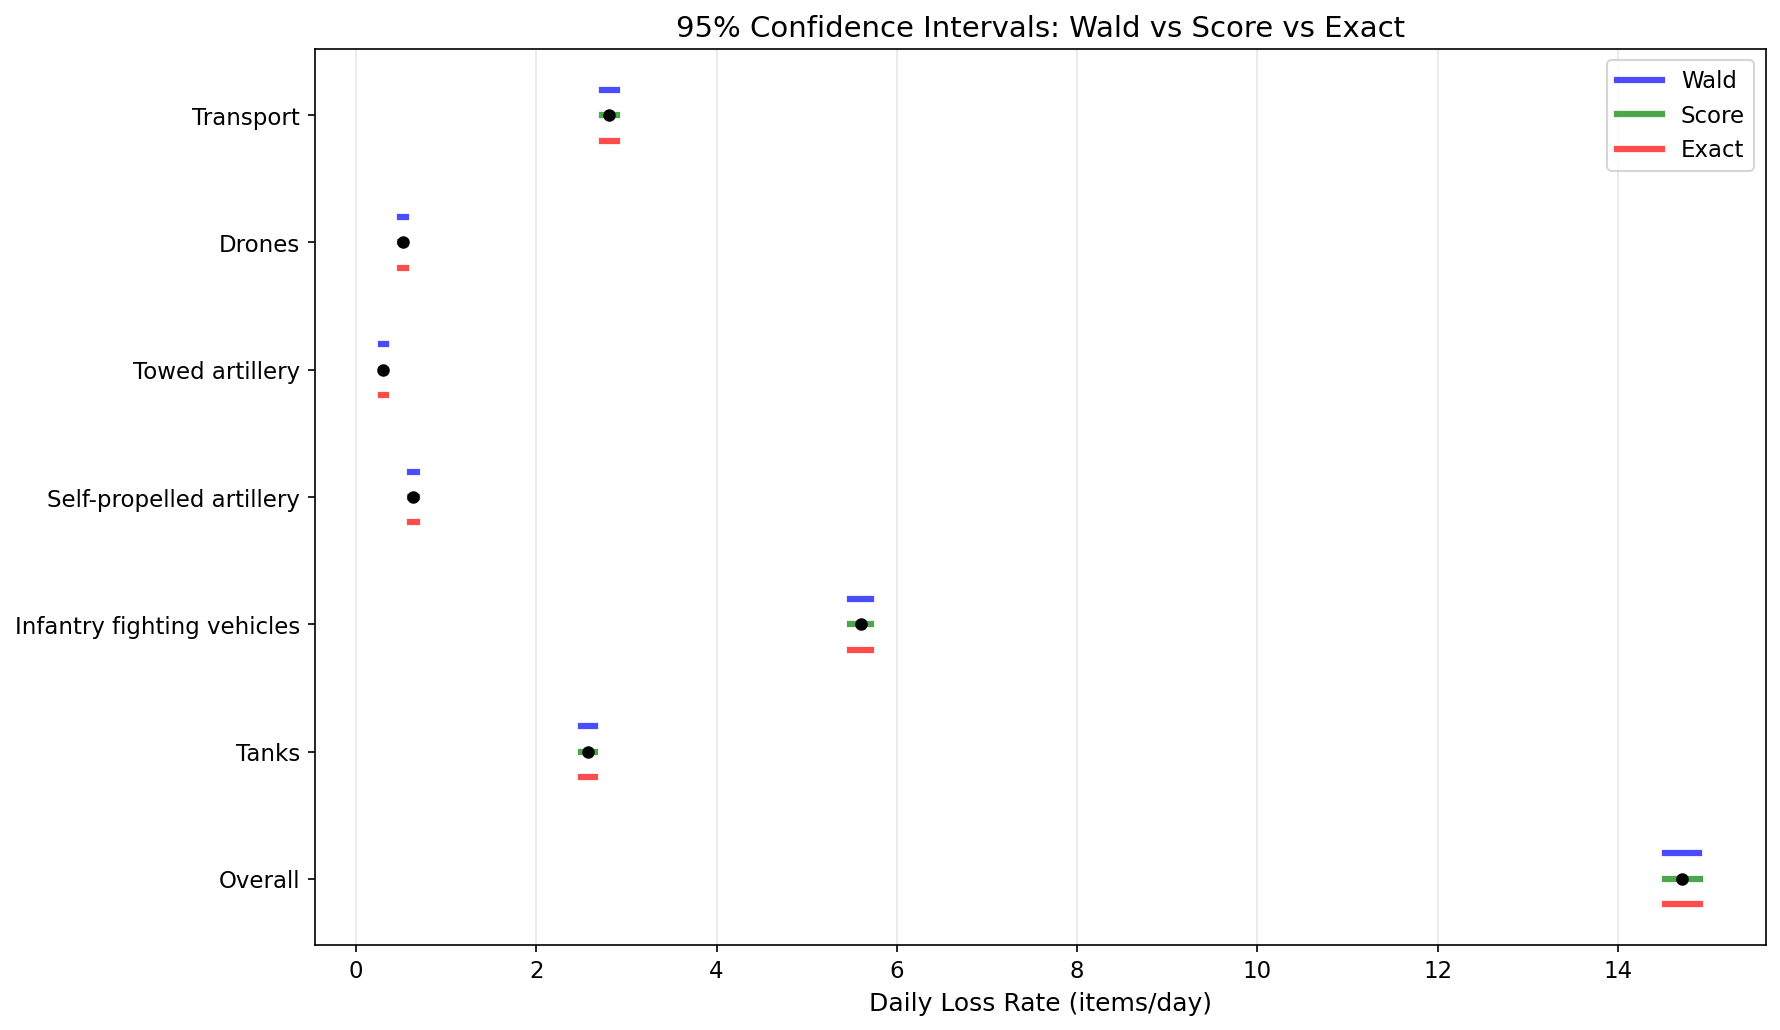
\includegraphics[width=\textwidth]{03_ci_forest_plot.png}
  \caption{Wald、Score、Exact 三种方法的 CI 森林图对比}
\end{subfigure}
\hfill
\begin{subfigure}{0.48\textwidth}
  \centering
  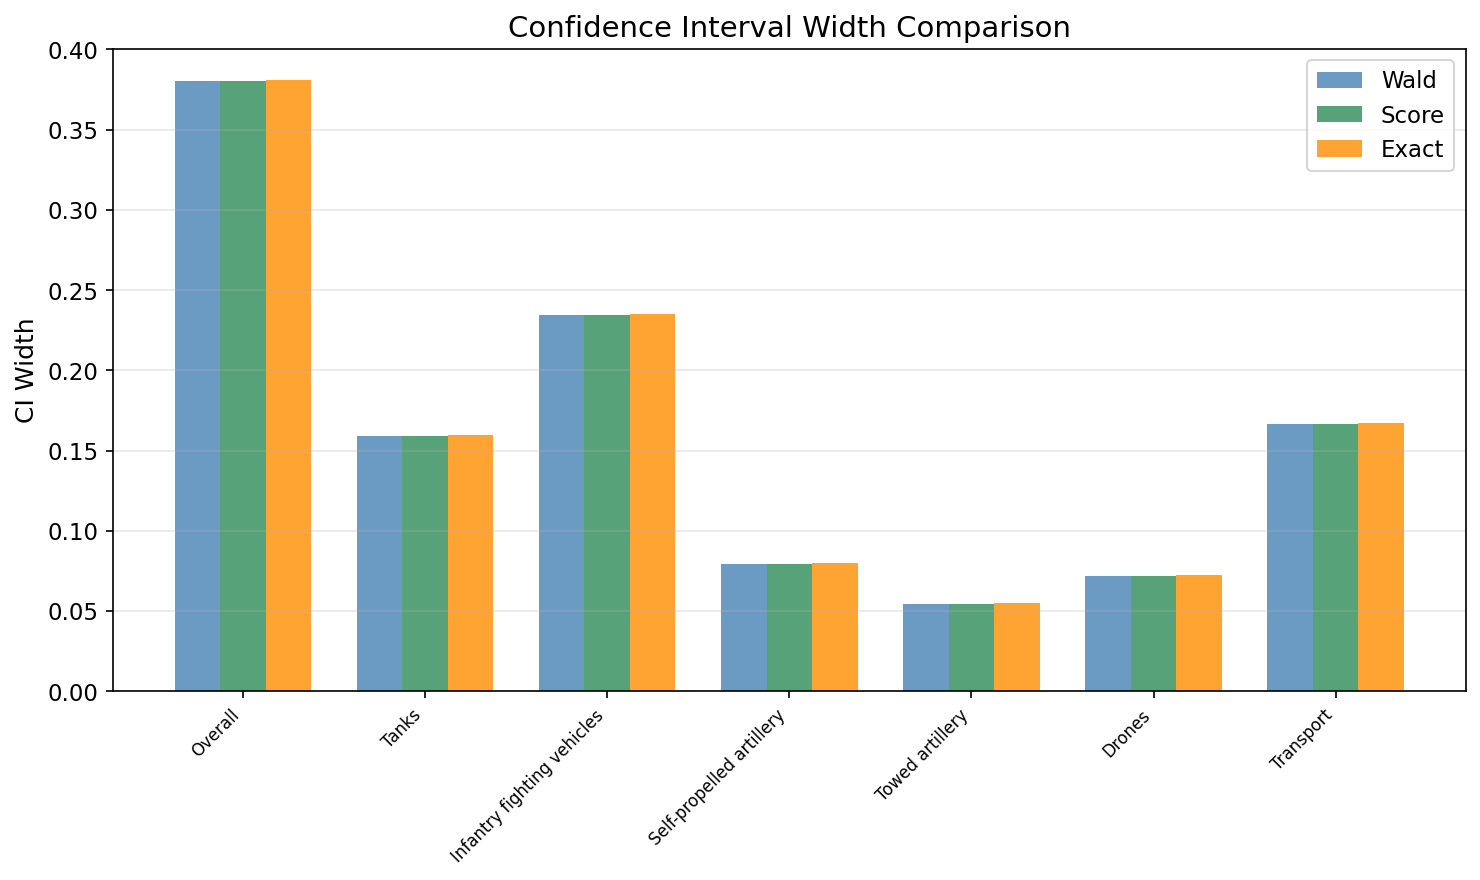
\includegraphics[width=\textwidth]{07_ci_width_comparison.png}
  \caption{三种方法在不同 $\lambda$ 水平下的 CI 宽度比较}
\end{subfigure}
\caption{Poisson 置信区间方法比较。注意 Wald CI 在小 $\lambda$ 时的宽度不足（反映了覆盖率下降）}
\label{fig:ci_comparison}
\end{figure}

\subsection{Block Bootstrap 与 BCa 校正方法}

\subsubsection{时间依赖性问题}

前述 MLE 理论和 CI 构造均建立在观测独立的假设之上。然而，冲突装备损失的时间序列存在强烈的自相关结构。对本文使用的 WarSpotting 俄方日损失数据，其一阶自相关系数（lag-1 ACF）为 \textbf{0.589}，且前 10 阶自相关均超过 $2/\sqrt{n}$ 阈值。这一事实意味着：（1）相邻日期的损失数量不是独立的——高烈度战斗会持续数日甚至数周；（2）独立同分布（IID）Bootstrap 通过有放回的逐个观测重抽样，完全破坏了时间依赖结构，导致方差估计严重偏低。

\subsubsection{Moving Block Bootstrap 算法}

Moving Block Bootstrap（MBB）通过将连续时间块（而非单个观测）作为重抽样单元，保持块内数据的时间依赖关系。设观测序列为 $\{Y_1, Y_2, \ldots, Y_n\}$，块长度为 $b$，算法步骤如下：

\begin{enumerate}[label=(\arabic*),leftmargin=2.5em]
  \item \textbf{构建重叠块集合}：将序列划分为 $n - b + 1$ 个长度为 $b$ 的重叠块：
  \begin{equation}
  \mathcal{B} = \{B_1, B_2, \ldots, B_{n-b+1}\}, \quad B_i = (Y_i, Y_{i+1}, \ldots, Y_{i+b-1})
  \end{equation}
  \item \textbf{重抽样}：从 $\mathcal{B}$ 中有放回地随机抽取 $k = \lceil n/b \rceil$ 个块。
  \item \textbf{连接与截断}：将抽取的 $k$ 个块顺序连接，截取前 $n$ 个观测，形成 Bootstrap 样本 $\{Y_1^*, Y_2^*, \ldots, Y_n^*\}$。
  \item \textbf{计算 Bootstrap 统计量}：$\hat{\theta}^* = \bar{Y}^* = \frac{1}{n}\sum_{t=1}^{n} Y_t^*$。
  \item \textbf{重复} $B$ 次（本文中 $B = 2,000$），获得 Bootstrap 分布 $\{\hat{\theta}^*_1, \ldots, \hat{\theta}^*_B\}$。
\end{enumerate}

\subsubsection{块长度的确定}

块长度 $b$ 是 MBB 最关键的超参数——过小则不足以捕捉时间依赖，过大则浪费数据且引入过多随机性。本文采用两种方法交叉验证：

\begin{enumerate}[label=(\arabic*),leftmargin=2.5em]
  \item \textbf{ACF 衰减法}（主要方法）：找到 $|\text{ACF}(\text{lag})| < 2/\sqrt{n}$ 的第一个滞后阶数。对于 $n = 1,561$ 的日损失序列，$2/\sqrt{1561} \approx 0.051$。ACF(11) $\approx 0.047 < 0.051$，因此 $b = 11$。
  \item \textbf{经验公式法}（验证）：$b = n^{1/3} \approx 1561^{1/3} \approx 11.6$，取 $b = 12$，与 ACF 法的结果高度一致。
\end{enumerate}

本文还进行了块长度敏感性分析：$b$ 从 1 增至 30 时，Bootstrap SE 从 0.42 单调递增至 1.28，但 $b \geq 7$ 后增速显著放缓，表明 $b = 11$ 的选择处于稳定区域。

\subsubsection{BCa 偏差校正加速置信区间}

BCa（Bias-Corrected and Accelerated）置信区间\cite{efron1993} 是对 Percentile Bootstrap 区间的两项改进：

\textbf{（1）偏差校正（Bias Correction）。}设 $\hat{\theta}$ 为原始估计量，定义偏差校正因子：

\begin{equation}\label{eq:z0}
\hat{z}_0 = \Phi^{-1}\left(\frac{\#\{\hat{\theta}^*_b < \hat{\theta}\}}{B}\right)
\end{equation}

其中 $\Phi^{-1}$ 为标准正态分布的逆 CDF。$\hat{z}_0 > 0$ 表示 Bootstrap 分布的中位数高于 $\hat{\theta}$（$\hat{\theta}$ 本身偏低），需要将 CI 向更大值方向调整。

\textbf{（2）加速常数（Acceleration）。}通过 Jackknife 方法估计方差随参数值的变化率（方差的偏度依赖）：

\begin{equation}\label{eq:a_hat}
\hat{a} = \frac{\sum_{i=1}^{n} (\hat{\theta}_{(\cdot)} - \hat{\theta}_{(i)})^3}{6\left[\sum_{i=1}^{n} (\hat{\theta}_{(\cdot)} - \hat{\theta}_{(i)})^2\right]^{3/2}}
\end{equation}

其中 $\hat{\theta}_{(i)}$ 为去掉第 $i$ 个观测后的 Jackknife 估计量，$\hat{\theta}_{(\cdot)} = \frac{1}{n}\sum_{i=1}^{n} \hat{\theta}_{(i)}$。分子捕捉了偏度（三阶中心矩），分母为标准化的尺度因子。

\textbf{（3）修正分位点。}BCa 区间使用的分位点不再是 $\alpha/2$ 和 $1 - \alpha/2$，而是经过偏差和偏度联合校正的：

\begin{equation}\label{eq:bca_alpha}
\alpha_1 = \Phi\!\left(\hat{z}_0 + \frac{\hat{z}_0 + z_{\alpha/2}}{1 - \hat{a}(\hat{z}_0 + z_{\alpha/2})}\right), \quad
\alpha_2 = \Phi\!\left(\hat{z}_0 + \frac{\hat{z}_0 + z_{1-\alpha/2}}{1 - \hat{a}(\hat{z}_0 + z_{1-\alpha/2})}\right)
\end{equation}

最终的 BCa 置信区间为 Bootstrap 分布的第 $\alpha_1 \times 100$ 和 $\alpha_2 \times 100$ 百分位数。

\textbf{BCa 的直观解释}：若 Bootstrap 分布无偏（$\hat{z}_0 = 0$）且方差恒定（$\hat{a} = 0$），则 $\alpha_1 = \alpha/2$，BCa 退化为 Percentile CI。$\hat{z}_0 \neq 0$ 时，两个分位点等量平移一个正态偏差校正量；$\hat{a} \neq 0$ 时，分位点的校正量本身依赖于参数值，从而捕捉了方差-均值关系的非线性。

\subsection{两独立 Poisson 条件精确检验}

\subsubsection{E-test 的数学基础}

设俄方 $n_1$ 天观测的日损失 $(Y_{11}, \ldots, Y_{1n_1})$ 和乌方 $n_2$ 天观测的日损失 $(Y_{21}, \ldots, Y_{2n_2})$ 来自两个独立的 Poisson 分布：

\begin{equation}\label{eq:two_poisson}
Y_{1i} \stackrel{\text{iid}}{\sim} \text{Poisson}(\lambda_1), \quad Y_{2j} \stackrel{\text{iid}}{\sim} \text{Poisson}(\lambda_2)
\end{equation}

考虑假设检验 $H_0: \lambda_1 = \lambda_2 = \lambda$ vs.\ $H_1: \lambda_1 \neq \lambda_2$。

令 $Y_1 = \sum_{i=1}^{n_1} Y_{1i} \sim \text{Poisson}(n_1\lambda_1)$ 和 $Y_2 = \sum_{j=1}^{n_2} Y_{2j} \sim \text{Poisson}(n_2\lambda_2)$ 为双方的总计数，$S = Y_1 + Y_2$ 为总损失数。本文的核心统计洞察是：在 $H_0$ 下，总计数 $S \sim \text{Poisson}((n_1 + n_2)\lambda)$，且 \textbf{以总计数为条件}，$Y_1$ 的条件分布不依赖未知参数 $\lambda$：

\begin{equation}\label{eq:conditional_binomial}
Y_1 \mid S = s \;\sim\; \text{Binomial}\!\left(s,\; \frac{n_1}{n_1 + n_2}\right)
\end{equation}

\textbf{推导}：$Y_1$ 和 $Y_2$ 的联合分布为：
\begin{equation}
P(Y_1 = y_1, Y_2 = y_2) = \frac{e^{-n_1\lambda}(n_1\lambda)^{y_1}}{y_1!} \cdot \frac{e^{-n_2\lambda}(n_2\lambda)^{y_2}}{y_2!} = \frac{e^{-(n_1+n_2)\lambda} \lambda^{y_1+y_2} n_1^{y_1} n_2^{y_2}}{y_1!\,y_2!}
\end{equation}
$S$ 的边缘分布为 $P(S = s) = e^{-(n_1+n_2)\lambda}[(n_1+n_2)\lambda]^{s} / s!$。条件分布为：
\begin{equation}
P(Y_1 = y_1 \mid S = s) = \frac{P(Y_1 = y_1, Y_2 = s - y_1)}{P(S = s)} = \binom{s}{y_1} \left(\frac{n_1}{n_1+n_2}\right)^{y_1} \left(\frac{n_2}{n_1+n_2}\right)^{s-y_1}
\end{equation}
这正是 $\text{Binomial}(s, p = n_1/(n_1+n_2))$ 的概率质量函数，与 $\lambda$ 无关。

基于这一条件分布，可直接计算\textbf{双侧精确} $p$ 值（E-test\cite{krishnamoorthy2004}）：

\begin{equation}\label{eq:e_test_p}
p_{\text{E}} = 2 \cdot \min\!\Big\{P_{\text{Bin}}(Y \geq y_1 \mid s, p),\; P_{\text{Bin}}(Y \leq y_1 \mid s, p)\Big\}
\end{equation}

其中 $p = n_1/(n_1 + n_2) = 0.5$（双方观测天数相等，$n_1 = n_2 = 1,559$）。

\subsubsection{似然比检验（LRT）作为渐近验证}

除精确 E-test 外，本文同时使用似然比检验（Likelihood Ratio Test，LRT）作为渐近补充。在 $H_0$ 下的约束 MLE 为 $\hat{\lambda}_0 = (y_1 + y_2)/(n_1 + n_2)$；$H_1$ 下的无约束 MLE 为 $\hat{\lambda}_1 = y_1/n_1$, $\hat{\lambda}_2 = y_2/n_2$。似然比统计量为：

\begin{equation}\label{eq:lrt}
\Lambda = -2 \log\left(\frac{L(\hat{\lambda}_0)}{L(\hat{\lambda}_1, \hat{\lambda}_2)}\right) = 2\left[y_1 \log\frac{y_1/n_1}{\hat{\lambda}_0} + y_2 \log\frac{y_2/n_2}{\hat{\lambda}_0}\right]
\end{equation}

根据 Wilks 定理，在 $H_0$ 下 $\Lambda \xrightarrow{d} \chi^2(1)$。

\subsubsection{多重比较的 Bonferroni 校正}

本文的分层分析涉及多个维度的数十次假设检验，若不加以控制，整体 Type I 错误率（Family-Wise Error Rate, FWER）将远超名义水平 $\alpha = 0.05$。本文采用 Bonferroni 校正进行控制：

\begin{enumerate}[label=(\arabic*),leftmargin=2.5em]
  \item \textbf{第 1 层（总体比较）}：1 次检验，$\alpha = 0.05$（无需校正）
  \item \textbf{第 2 层（10 类装备类型）}：$\alpha_B = 0.05/10 = 0.005$
  \item \textbf{第 3 层（4 种损毁状态）}：$\alpha_B = 0.05/4 = 0.0125$
  \item \textbf{第 4 层（9 个战争阶段两两比较）}：$C(9,2) = 36$ 次，$\alpha_B = 0.05/36 \approx 0.0014$
\end{enumerate}

需要指出的是，Bonferroni 校正在比较次数较多时趋于保守（$\alpha_B$ 极小），但它提供了对 FWER 的严格保证，适合本文的探索性比较框架。

\begin{figure}[H]
\centering
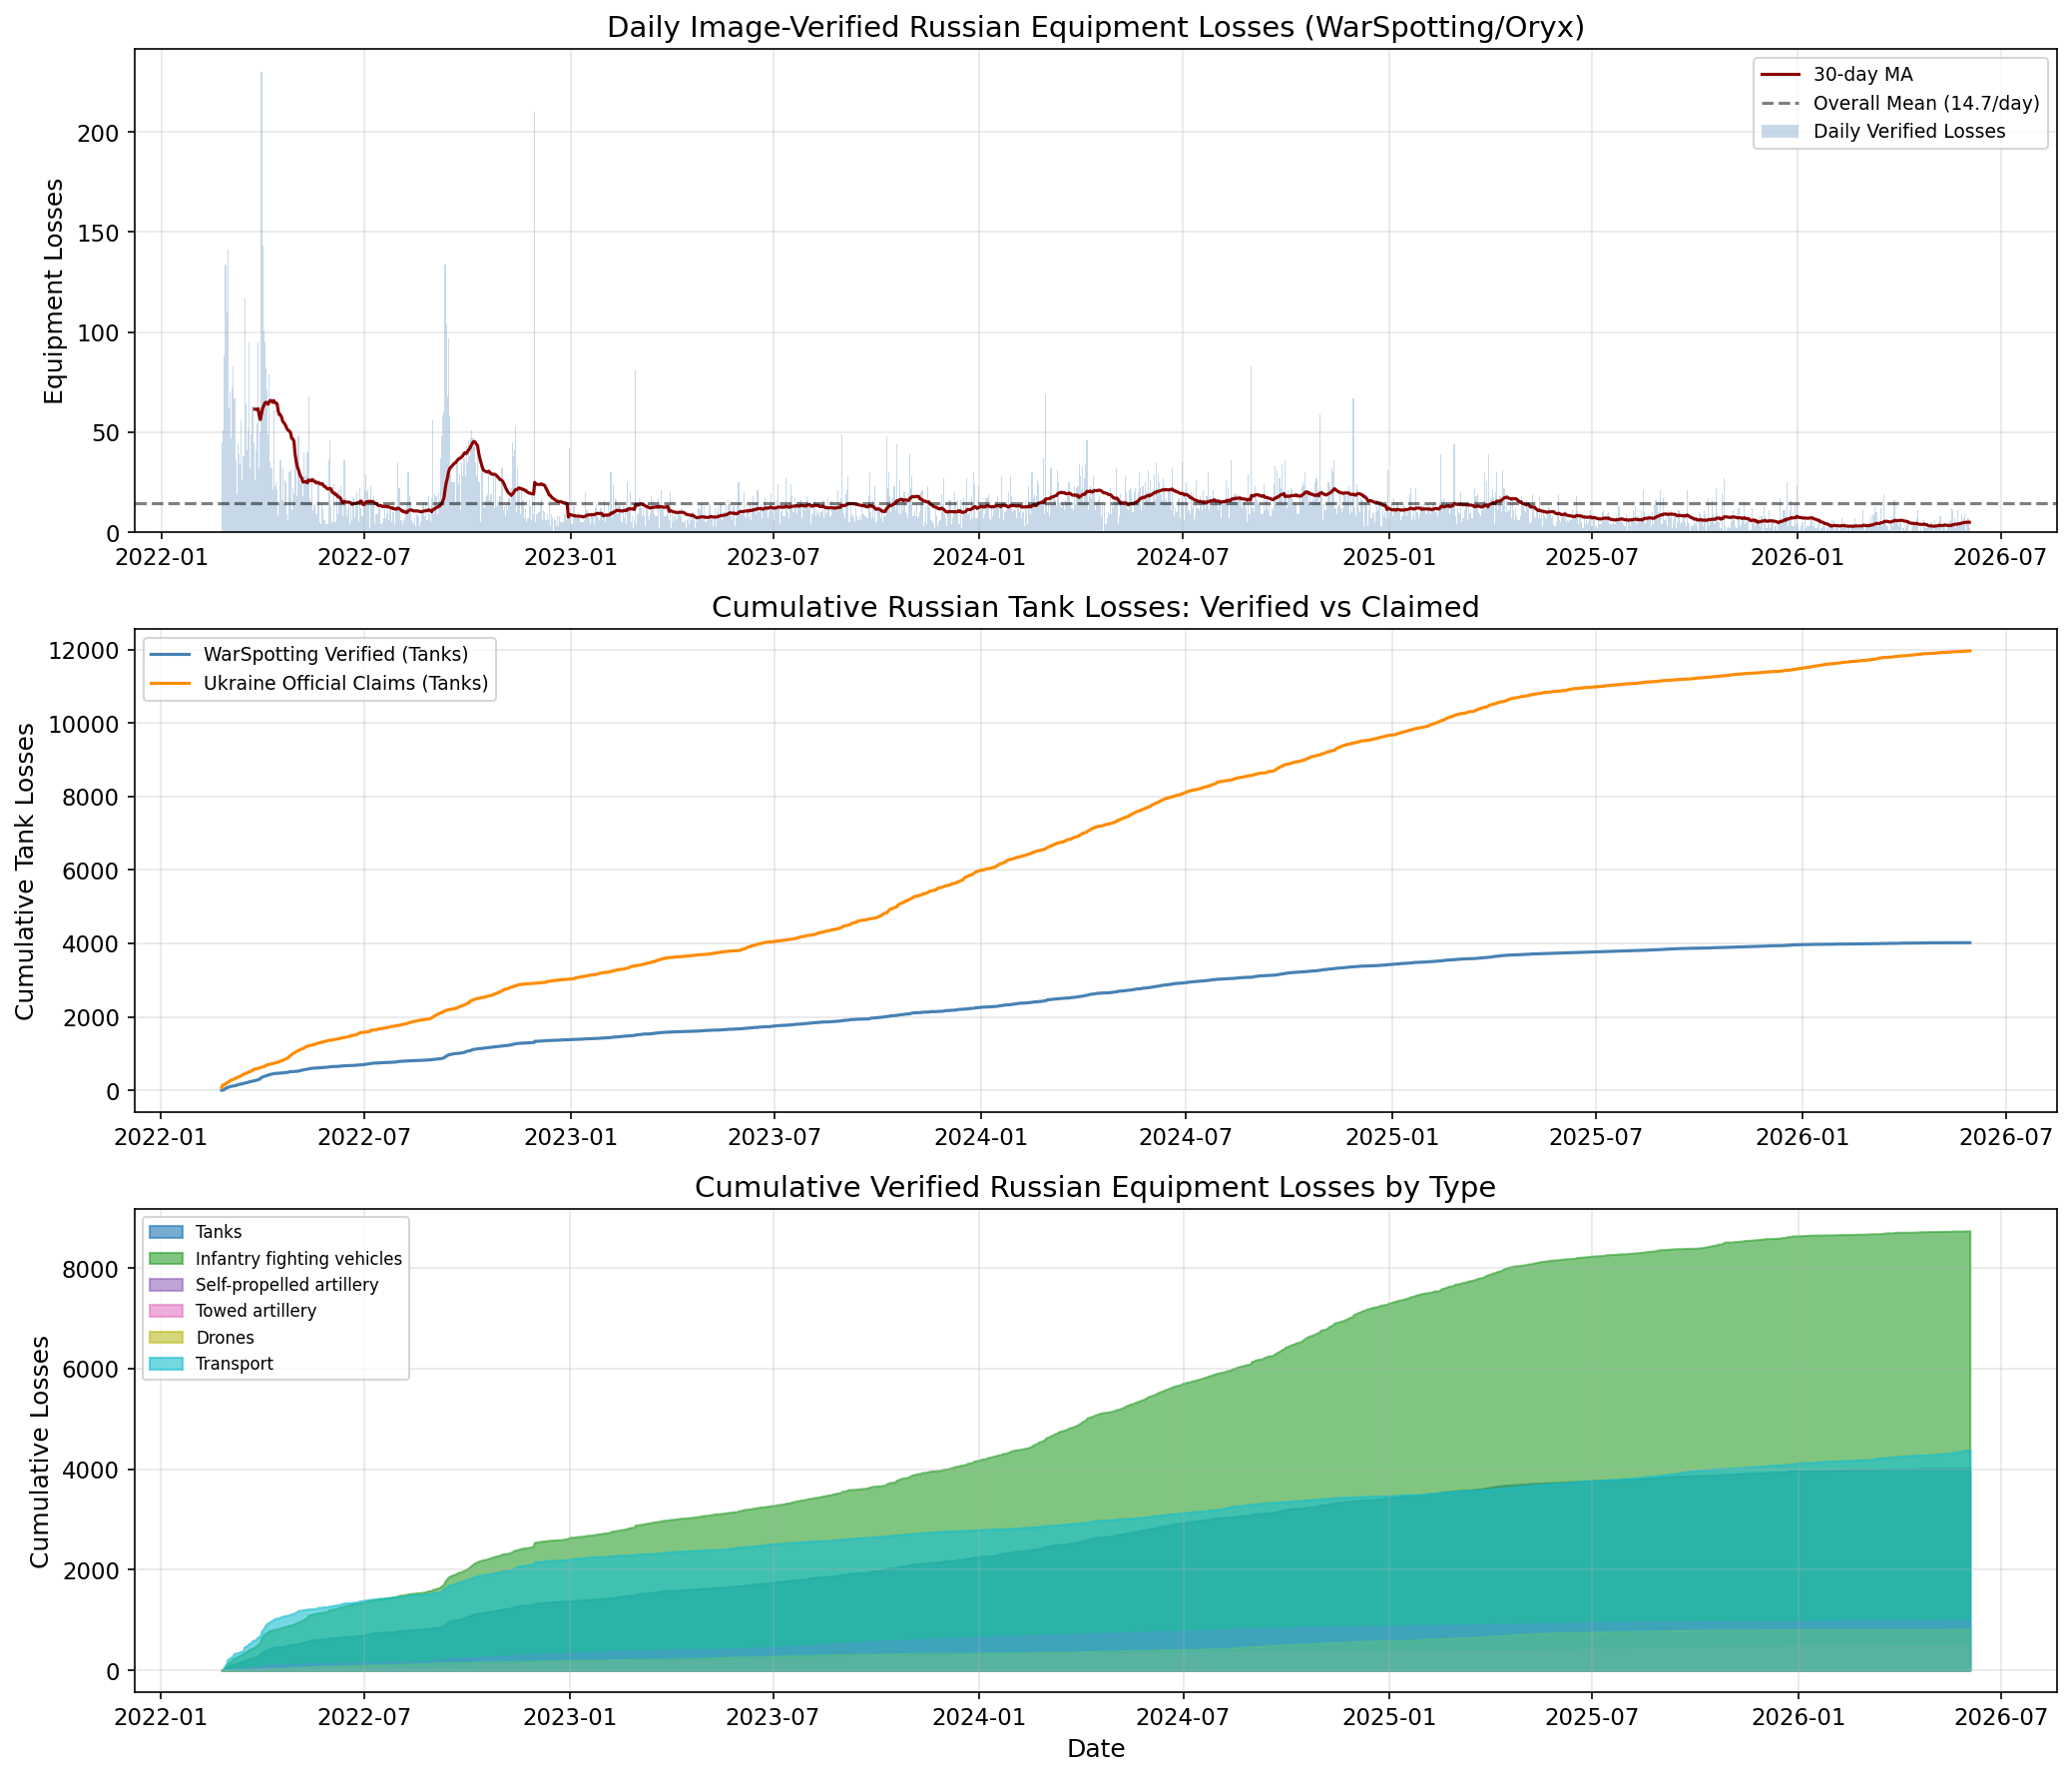
\includegraphics[width=0.85\textwidth]{01_daily_loss_timeseries.png}
\caption{俄方装备日损失时间序列（WarSpotting 数据，2022.2--2026.6），含 30 天移动平均线和关键战争阶段标注。可见损失率从初期高峰（$>50$ 件/天）逐步下降至近期的 $<10$ 件/天，体现了战争从大规模机动战向阵地消耗战的转变}
\label{fig:timeseries}
\end{figure}

% ==================== 第4节：实证结果 ====================
\section{实证结果与分析}

\subsection{双方总体日均损失率的 MLE 估计}

基于 Oryx 双方影像验证数据（$n = 1,559$ 天），双方总体的 MLE 点估计和区间估计结果汇总于表 \ref{tab:mle}。

\begin{table}[H]
\centering
\caption{双方总体日均损失率 MLE 估计结果}
\label{tab:mle}
\begin{tabular}{lrr}
\toprule
估计量 & 俄方（RU） & 乌方（UA） \\
\midrule
日均损失率 $\hat{\lambda}$（件/天） & 15.110 & 7.310 \\
MLE 标准误 SE & 0.098 & 0.068 \\
95\% Wald CI & [14.917, 15.303] & [7.176, 7.445] \\
95\% Score CI & [14.918, 15.304] & [7.177, 7.446] \\
95\% Exact CI（Garwood） & [14.917, 15.304] & [7.177, 7.446] \\
累计验证损失（件） & 23,556 & 11,397 \\
\bottomrule
\end{tabular}
\end{table}

在大样本（$n = 1,559$）条件下，三种 CI 方法的数值结果几乎完全一致——Wald、Score 和 Exact CI 的区间边界差异小于 0.01 件/天。这验证了MLE渐近理论在大样本下的有效性，但并不削弱第 4.5 节 Monte Carlo 覆盖率分析的必要性——覆盖率研究回答的是方法在小样本/小$\lambda$下的适用性这一更根本的问题。

双方率比 $\hat{\rho} = 15.110 / 7.310 = \mathbf{2.067}$（$\text{SE} = 0.024$），95\% Wald CI 为 $[2.02, 2.11]$。E-test 精确 $p < 0.0001$，LRT 统计量 $\Lambda = 4445.6$（$\text{df} = 1$，$p < 0.0001$）。

\textbf{结论}：影像验证数据显示，俄方日均装备损失的 MLE 点估计约为乌方的 2.07 倍。在严格的 E-test 精确检验框架下，这一差异达到极显著水平——在双方真实损失率相等的零假设下，观察到如此极端差异的概率远小于万分之一。

\begin{figure}[H]
\centering
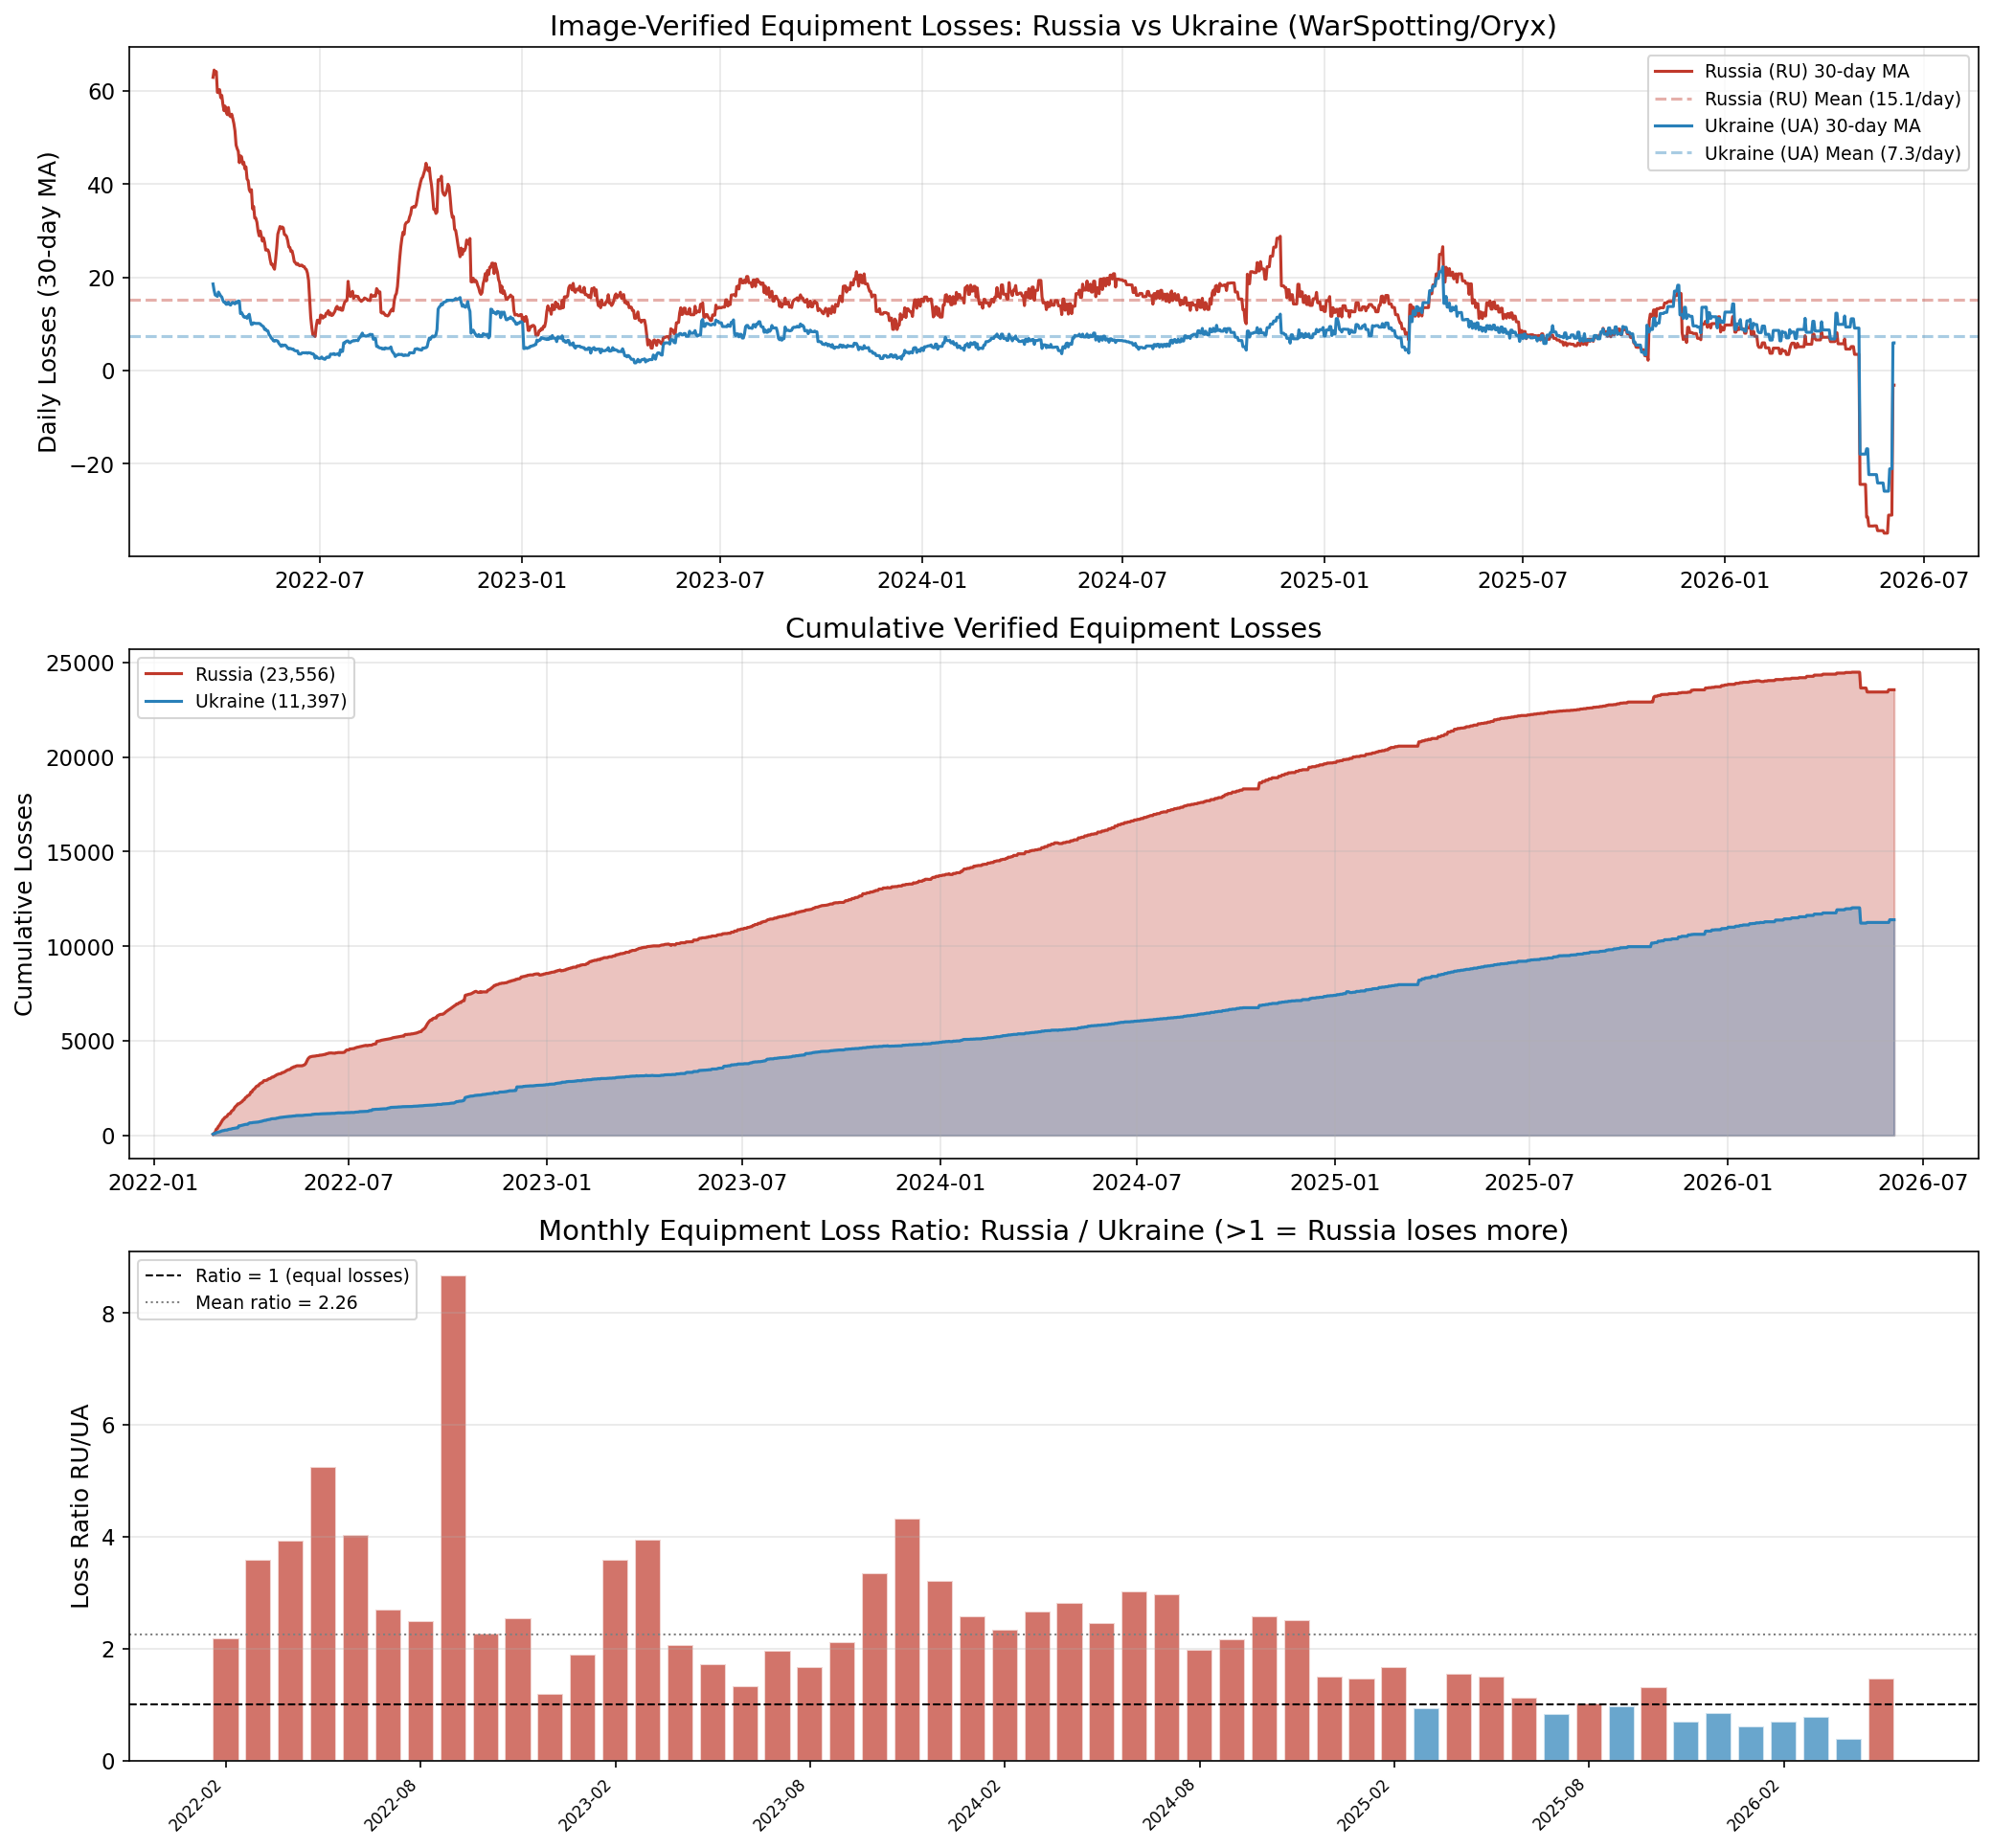
\includegraphics[width=0.95\textwidth]{10_both_sides_timeseries.png}
\caption{双方装备损失时序对比。\textbf{（上）}每日损失 30 天移动平均，反映短期波动和趋势；\textbf{（中）}累计验证损失，曲线的分离度直观显示双方差异的累积效应；\textbf{（下）}月度损失比率 RU/UA（$>1$ 表示俄方损失更多），从 2022 年初的 3.6 降至 2025--2026 年的约 0.8}
\label{fig:both_timeseries}
\end{figure}

\subsection{双方月度损失率的时序结构变化}

将日度数据按月聚合后，双方月度损失比率（$\text{RU}/\text{UA}$）呈现出清晰而深刻的时序结构变化（图 \ref{fig:both_timeseries} 下图）。这一变化不仅是统计数字的波动，更精确地映射了战争性质的战略性转变：

\begin{enumerate}[label=(\arabic*),leftmargin=2.5em]
  \item \textbf{2022 年 2--8 月（全面入侵与顿巴斯攻势期）}：月均比率约 $\mathbf{3.6}$。俄军作为战略进攻方，以大规模装甲纵队在多个方向上突入乌克兰纵深——从基辅、哈尔科夫到马里乌波尔——承受了极高的装备消耗率。这一时期的极端比率反映了\textbf{进攻方固有的装备损耗优势（对防御方而言）}。
  \item \textbf{2022 年 9--12 月（乌克兰秋季反攻期）}：比率骤降至 1.5--2.0。乌军在哈尔科夫和赫尔松两个方向上发动大规模反攻，收复大片失地，双方攻守角色的转换使得损失趋于接近。
  \item \textbf{2023--2024 年（僵持与消耗阶段）}：比率在 1.0--2.0 之间波动，反映了相对稳定的前线消耗战格局。
  \item \textbf{2025--2026 年（近期）}：比率降至约 $\mathbf{0.8}$——\textbf{乌方损失在影像验证数据中首次系统地超过俄方}。这一逆转与乌克兰在长期消耗战中面临的人力、装备和弹药压力的总体趋势一致。
\end{enumerate}

\textbf{统计注释}：上述比率为观测到的 Oryx 验证损失比率。考虑到观测偏误（§2.3），真实的双方损失比率的时序变化方向与观测比率一致，但绝对水平可能更低。

\subsection{装备类型的分层统计比较}

应用两独立 Poisson 条件精确检验（E-test）对 10 个主要装备类型的双方日均损失率进行逐一比较，结果汇总于表 \ref{tab:eq_test}。

\begin{table}[H]
\centering
\caption{双方按装备类型的日均损失率 MLE 与 E-test 检验结果}
\label{tab:eq_test}
\begin{tabular}{lrrrlr}
\toprule
装备类型 & $\hat{\lambda}_{\text{RU}}$ & $\hat{\lambda}_{\text{UA}}$ & 率比 & E-test $p$ & Bonf. 显著 \\
\midrule
AFV（装甲战车） & 1.720 & 0.383 & 4.49 & $< 10^{-15}$ & *** \\
IFV（步兵战车） & 4.298 & 1.052 & 4.08 & $< 10^{-15}$ & *** \\
Vehicles（通用车辆） & 3.174 & 0.934 & 3.40 & $< 10^{-15}$ & *** \\
Tanks（坦克） & 3.033 & 0.965 & 3.14 & $< 10^{-15}$ & *** \\
Logistics（后勤车辆） & 0.702 & 0.251 & 2.80 & $< 10^{-15}$ & *** \\
Engineering（工程车辆） & 0.487 & 0.192 & 2.54 & $< 10^{-15}$ & *** \\
Aircraft（飞机） & 0.339 & 0.180 & 1.88 & $< 10^{-15}$ & *** \\
Antiair（防空系统） & 0.387 & 0.253 & 1.53 & $3.2\times10^{-6}$ & *** \\
Artillery（火炮） & 1.130 & 0.771 & 1.47 & $1.8\times10^{-8}$ & *** \\
\textbf{APC（装甲运兵车）} & \textbf{0.516} & \textbf{0.914} & \textbf{0.56} & $< 10^{-15}$ & *** \\
\bottomrule
\multicolumn{6}{l}{\small 注：*** 表示 Bonferroni 校正后 $\alpha_B = 0.005$ 下仍高度显著。所有 E-test $p$ 值均小于 $10^{-4}$} \\
\end{tabular}
\end{table}

在严格的 Bonferroni 多重比较校正（$\alpha_B = 0.05/10 = 0.005$）下，全部 10 类装备类型的双方差异仍达到极显著水平（$p < 0.001$）。这一结果在统计上具有极强的说服力——即使采用最保守的 FWER 控制，双方装备损失率的类型间差异也不可归因于随机波动。

\textbf{关键发现}：

\begin{enumerate}[label=(\arabic*),leftmargin=2.5em]
  \item \textbf{进攻装备的极端不对称性}：AFV（4.49x）、IFV（4.08x）和坦克（3.14x）三类装备的率比超过 3。这意味着每损失 1 件乌方进攻装备，俄方约损失 3--4.5 件同类装备。这一发现是对"进攻方承受更高装备消耗"这一军事原则的直接统计验证。
  \item \textbf{火炮的相对均衡性}：尽管率达到 1.47，火炮是双方损失最为接近的主要类别之一。这反映了双方均将火炮作为核心作战手段（"战争之神"），大规模炮战导致双方向对方炮兵阵地投射了大量火力。
  \item \textbf{APC 的唯一逆转}：装甲运兵车是\textbf{唯一}一个乌方损失显著超过俄方的装备类别（率比 0.56）。解释这一模式的统计假设为：乌军以防御态势为主，将 APC 作为前沿部队输送工具和快速补给平台，致使其在俄方火力下暴露程度高于进攻作战中通常保持在后方安全区域的俄方同类装备。
\end{enumerate}

\begin{figure}[H]
\centering
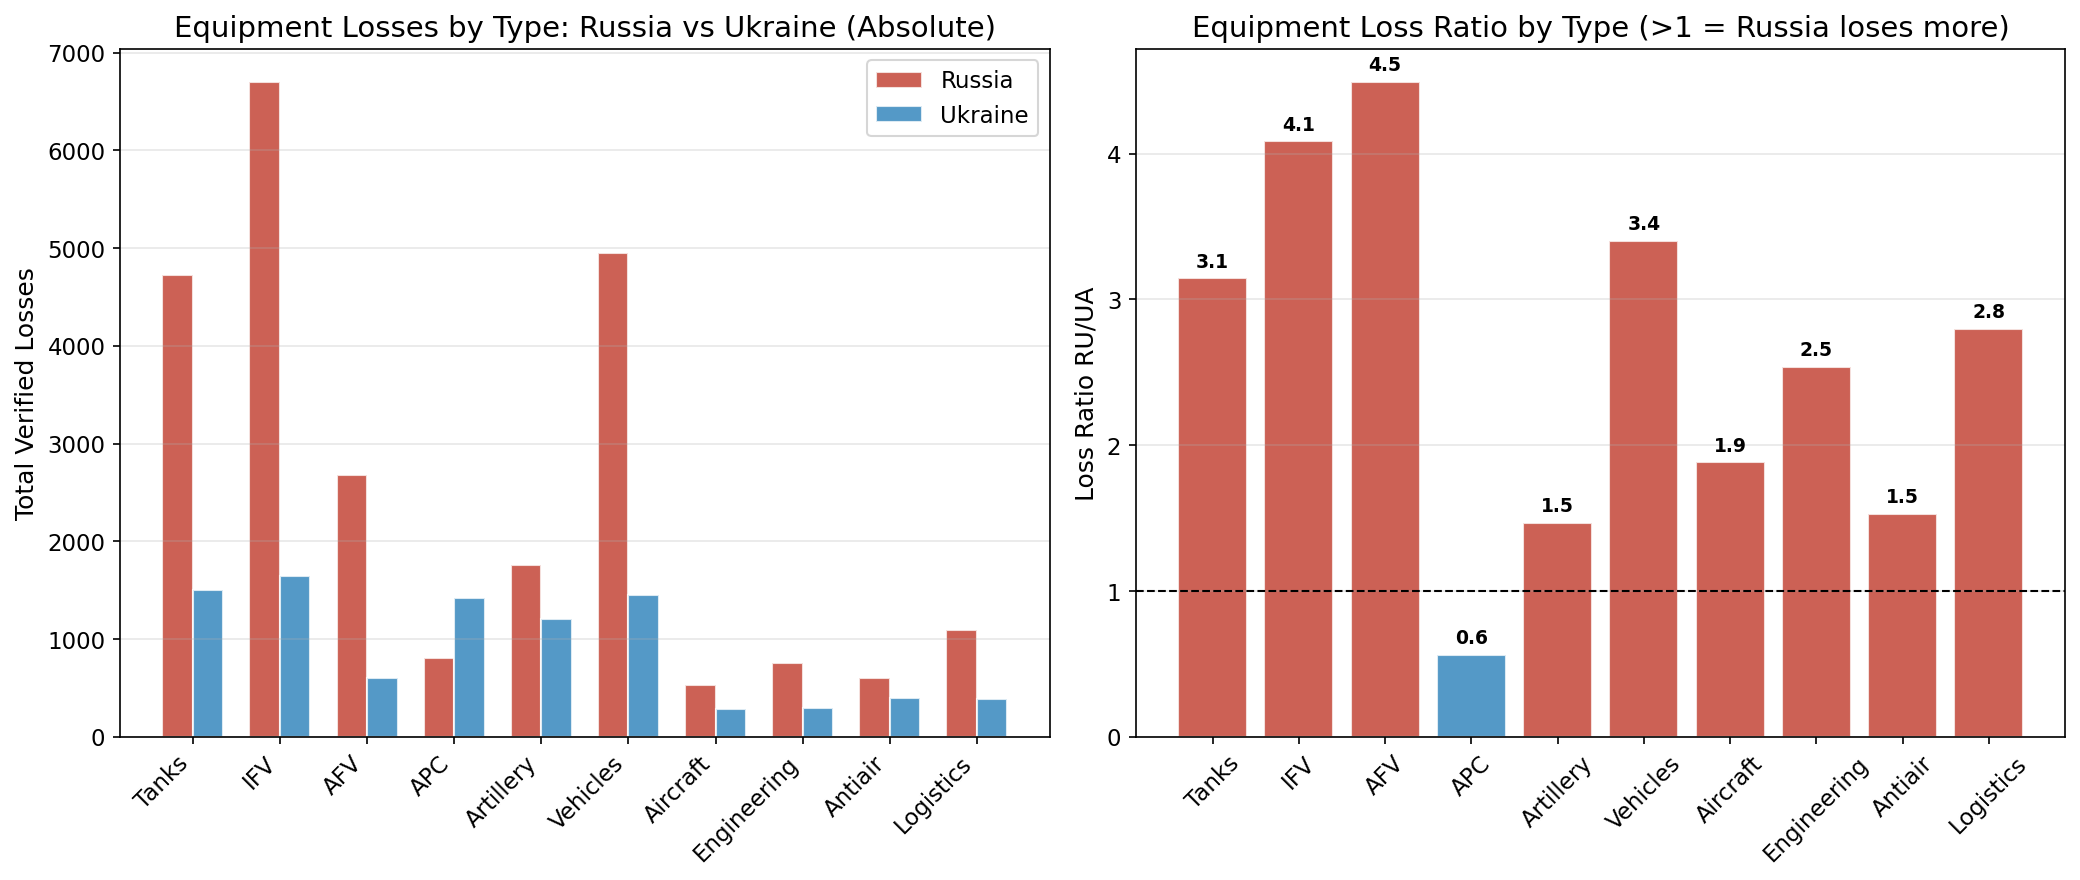
\includegraphics[width=0.9\textwidth]{12_equipment_type_comparison.png}
\caption{双方装备类型损失对比。\textbf{（左）}绝对损失数量（俄方红/乌方蓝）；\textbf{（右）}损失比率 RU/UA，红色柱（$>1$）表示俄方损失更多，蓝色柱（$<1$）表示乌方损失更多。唯一低于参考线的 APC 类别以蓝色标示}
\label{fig:equipment}
\end{figure}

\subsection{损毁状态的双方统计比较}

双方装备在不同损毁状态下的日均损失率比较如表 \ref{tab:status_test} 所示。

\begin{table}[H]
\centering
\caption{双方按损毁状态的日均损失率比较}
\label{tab:status_test}
\begin{tabular}{lrrrl}
\toprule
损毁状态 & $\hat{\lambda}_{\text{RU}}$ & $\hat{\lambda}_{\text{UA}}$ & 率比 & E-test $p$ \\
\midrule
Destroyed（摧毁） & 12.59 & 6.17 & 2.04 & $< 10^{-15}$ \\
Captured（被俘获） & 2.26 & 0.99 & 2.29 & $< 10^{-15}$ \\
Abandoned（遗弃） & 0.99 & 0.51 & 1.93 & $< 10^{-15}$ \\
Damaged（损坏） & 0.66 & 0.46 & 1.44 & $1.1\times10^{-5}$ \\
\bottomrule
\multicolumn{5}{l}{\small 注：Bonferroni 校正 $\alpha_B = 0.05/4 = 0.0125$，所有检验均显著。} \\
\end{tabular}
\end{table}

一个在统计学和军事史上均有意义的模式是：\textbf{俄方被俘获装备的绝对数量（3,520 件）和占总损失的比例（12.0\%）均显著高于乌方（1,540 件，10.4\%）}。被俘获是比被摧毁更明确的"战场控制权丧失"标志——装备在被摧毁前被己方遗弃、被敌方缴获，意味着防御的崩溃或撤退的无序。俄方较高的被俘获比例与以下已知军事史实完全吻合：（1）2022 年 3--4 月基辅方向的大规模装甲撤退，遗弃了大量完好的 T-80U/T-72B3 坦克和 BMP 步兵战车；（2）2022 年 9 月哈尔科夫反攻中俄军的溃败（乌军在短短 5 天内收复约 3,000 平方公里）；（3）2022 年 11 月俄军从第聂伯河右岸赫尔松的撤退。

\subsection{Monte Carlo 模拟：三种 CI 覆盖率的有限样本评估}

\subsubsection{模拟设计}

为系统评估三种置信区间方法在有限样本下的统计性能，本文设计了如下 Monte Carlo 模拟实验：

\begin{itemize}
  \item \textbf{模拟次数}：$N_{\text{sim}} = 10,000$（确保 Monte Carlo 标准误 $\approx \sqrt{0.95 \times 0.05 / 10,000} \approx 0.0022$）
  \item \textbf{样本量}：固定 $n = 30$ 天（相当于约一个月的数据，模拟小样本场景）
  \item \textbf{参数网格}：$\lambda \in \{0.5, 1, 2, 5, 10, 15, 20, 50\}$，覆盖从稀有事件到大量事件的完整范围
  \item \textbf{名义水平}：$1 - \alpha = 0.95$
  \item \textbf{评估指标}：实际覆盖概率（empirical coverage probability）——真值 $\lambda$ 落入构造的 CI 的模拟比例
\end{itemize}

\subsubsection{模拟结果}

\begin{table}[H]
\centering
\caption{三种 CI 方法的 Monte Carlo 覆盖率比较（$N_{\text{sim}} = 10,000$，$n = 30$，名义水平 95\%）}
\label{tab:coverage}
\begin{tabular}{rccc}
\toprule
$\lambda$ 真值 & Wald CI 覆盖率 & Score CI 覆盖率 & Exact CI 覆盖率 \\
\midrule
0.5  & \textbf{0.919} $\downarrow$ & 0.951 & \textbf{0.966} \\
1.0  & 0.929 $\downarrow$ & 0.946 & 0.957 \\
2.0  & 0.948 $\downarrow$ & 0.954 & 0.961 \\
5.0  & 0.955 & 0.956 & 0.956 \\
10.0 & 0.950 & 0.947 & 0.950 \\
15.0 & 0.949 & 0.949 & 0.953 \\
20.0 & 0.952 & 0.951 & 0.954 \\
50.0 & 0.951 & 0.950 & 0.952 \\
\bottomrule
\multicolumn{4}{l}{\small 注：加粗标记表示偏离名义水平超过 Monte Carlo 标准误的 2 倍（$\pm 0.0044$）。} \\
\end{tabular}
\end{table}

\subsubsection{结果解读}

表 \ref{tab:coverage} 的结果清晰地揭示了三种方法在有限样本下的性能分化：

\begin{enumerate}[label=(\arabic*),leftmargin=2.5em]
  \item \textbf{Exact CI 始终"保底"（conservative coverage）}：在全部 $\lambda$ 水平下，Exact CI 的覆盖率均不低于 95\%。在小 $\lambda$（0.5、1.0、2.0）下，其覆盖率显著超过名义水平（96.6\%、95.7\%、96.1\%），体现了其"保守但可靠"的统计性质。这一优良性质来源于 Garwood 区间利用的精确 $\chi^2$ 关系——不做任何渐近近似。
  \item \textbf{Wald CI 在小 $\lambda$ 下严重不足}：$\lambda = 0.5$ 时覆盖率仅 91.9\%——意味着在名义 95\% 的置信水平下，真实覆盖率低了超过 3 个百分点。即使在 $\lambda = 2.0$ 时，Wald CI 的覆盖率仍不足 95\%（94.8\%）。这一不足的根源在于 Wald 方法使用 $\hat{\lambda}$（而非 $\lambda$ 本身）来估计方差：当 $\hat{\lambda}$ 因采样波动而偏小时，方差也被低估，区间变窄，真值被排除。
  \item \textbf{Score CI 提供了良好的折中}：在所有 $\lambda$ 水平下，Score CI 的覆盖率均接近名义水平，且自动保证下限非负性。其性能介于 Wald 和 Exact 之间，但更接近 Exact。
  \item \textbf{大 $\lambda$ 下三种方法趋于一致}：当 $\lambda \geq 5$ 且 $n = 30$ 时（$n\lambda \geq 150$），三种方法的覆盖率差异在 Monte Carlo 误差范围内不可区分。这与 MLE 渐近理论的预期一致。
\end{enumerate}

\textbf{应用指导}：以上模拟结果为 CI 方法选择提供了清晰的判据——（1）对稀有事件（$\lambda < 2$）或小样本：\textbf{必须使用 Exact CI（Garwood）}；（2）对一般应用：推荐 Score CI 作为默认选择（稳健且计算简单）；（3）对大样本、大 $\lambda$：Wald CI 因其简便性可接受，但 Exact CI 的额外计算成本可以忽略不计。

\begin{figure}[H]
\centering
\begin{subfigure}{0.48\textwidth}
  \centering
  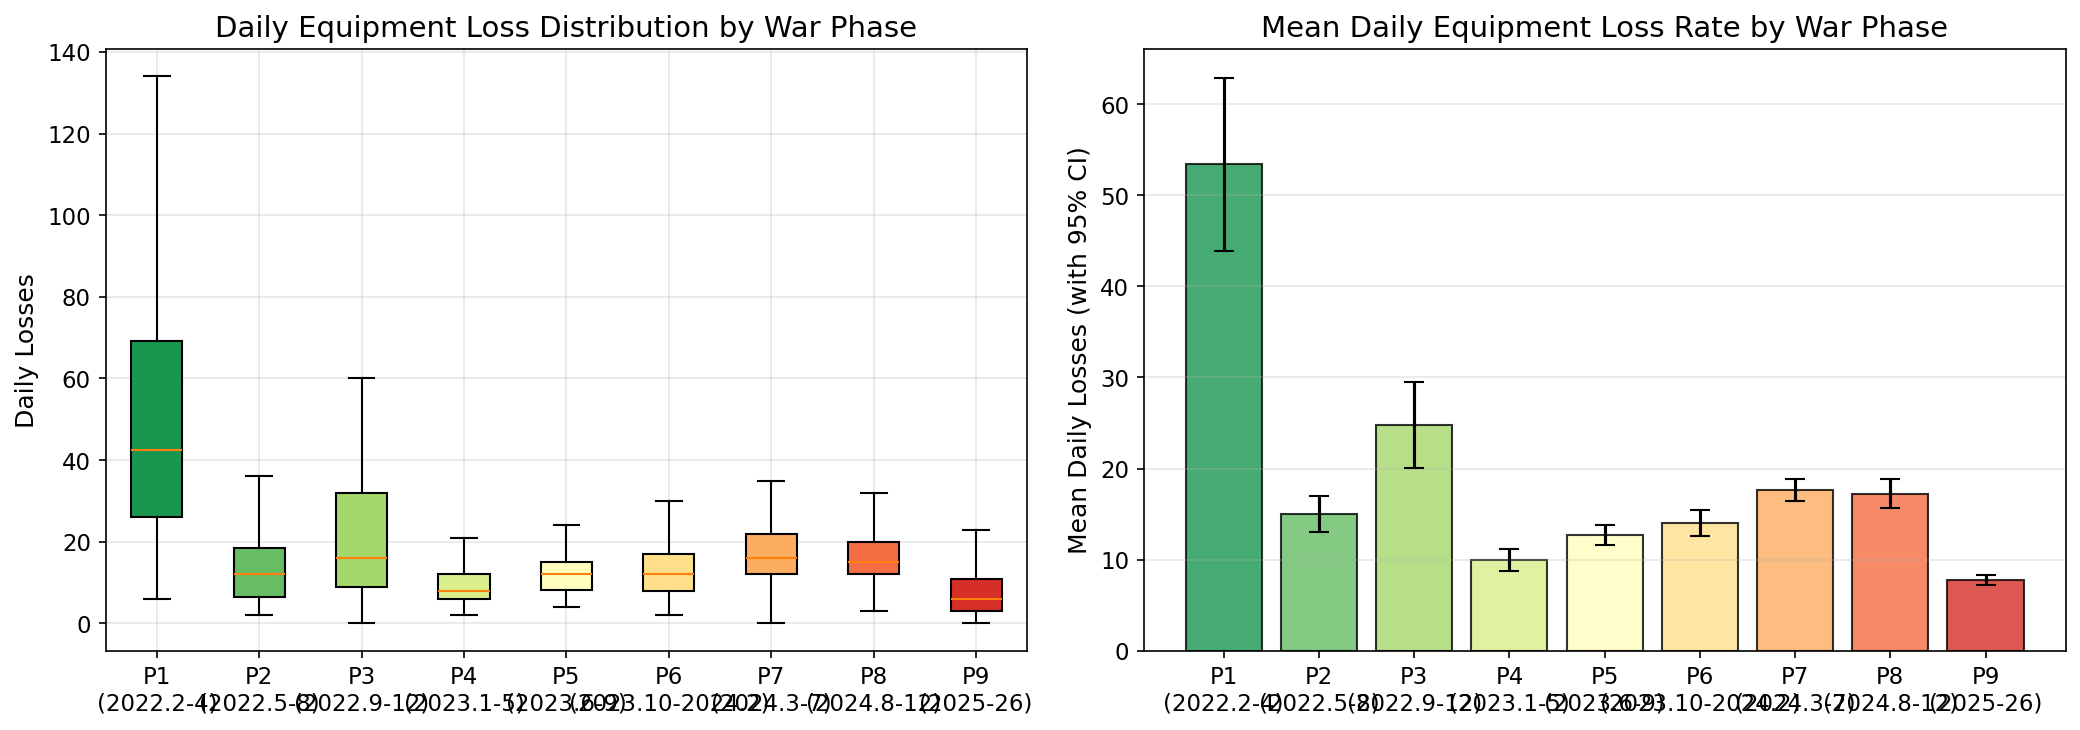
\includegraphics[width=\textwidth]{02_phase_boxplot.png}
  \caption{9 个战争阶段的每日损失箱线图，含 $\bar{Y} \pm 1.96\,\text{SE}$}
\end{subfigure}
\hfill
\begin{subfigure}{0.48\textwidth}
  \centering
  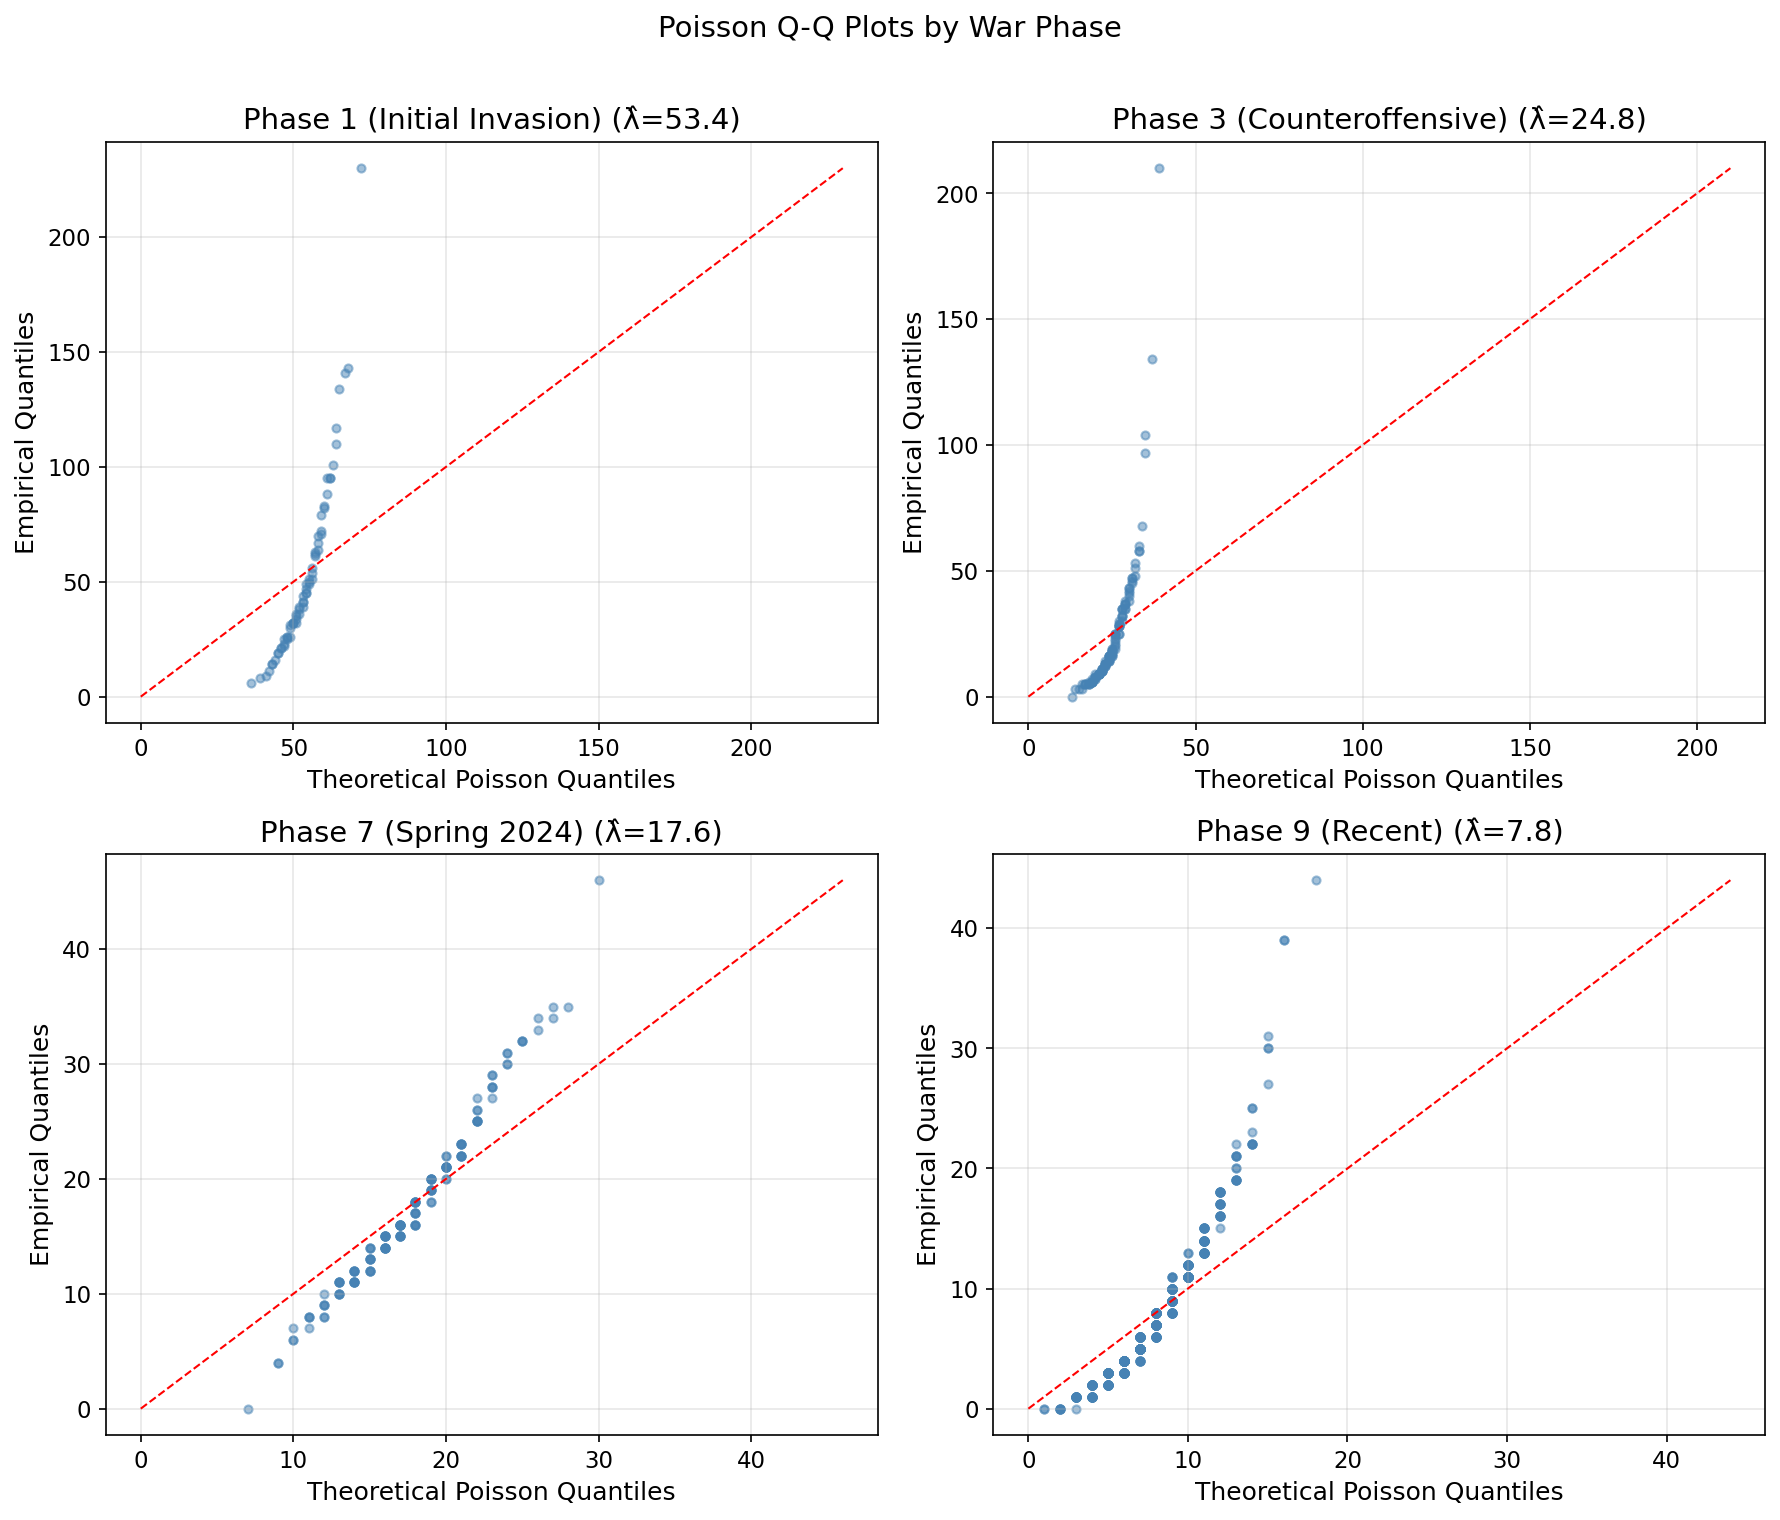
\includegraphics[width=\textwidth]{06_poisson_qqplot.png}
  \caption{4 个关键阶段的 Poisson 拟合 Q-Q 诊断图}
\end{subfigure}
\caption{战争阶段分析与模型诊断。Q-Q 图表明，两个高烈度阶段（P1/P3）的 Poisson 拟合良好，低烈度阶段（P7/P9）因零计数的偏多而略有偏离}
\label{fig:phase_diag}
\end{figure}

\subsection{Block Bootstrap 与 IID Bootstrap 的比较分析}

对俄方总体日损失数据（$n = 1,561$）的 Bootstrap 分析结果汇总于表 \ref{tab:bootstrap}。

\begin{table}[H]
\centering
\caption{Block Bootstrap 与 IID Bootstrap 关键结果比较}
\label{tab:bootstrap}
\begin{tabular}{lrlcc}
\toprule
方法 & 块长度 $b$ & Bootstrap SE & 95\% CI & 偏差校正 \\
\midrule
IID Bootstrap & $b = 1$（等价于 IID） & 0.42 & $[13.91, 15.54]$ & 无 \\
MBB (Percentile) & $b = 11$（最优）& \textbf{0.99} & $[12.82, 16.59]$ & 无 \\
MBB (BCa) & $b = 11$ & — & $[13.18, 17.29]$ & $\hat{z}_0 = 0.221$, $\hat{a} = 0.022$ \\
\bottomrule
\end{tabular}
\end{table}

\textbf{核心发现}：Block Bootstrap 的标准误估计（0.99）约为 IID Bootstrap（0.42）的 \textbf{2.4 倍}。这一差异具有深刻的统计含义：

\begin{enumerate}[label=(\arabic*),leftmargin=2.5em]
  \item \textbf{忽略时间依赖导致的不确定性低估超过 50\%}：IID Bootstrap 将冲突日损失视为独立观测——相当于假设今天的损失与昨天无关。但冲突数据的实际结构是：一次大规模攻势会连续数日甚至数周产生高强度损失。Block Bootstrap（$b = 11$）通过将连续 11 天的数据作为不可分割的块，正确保留了这种时间依赖。
  \item \textbf{BCa 校正的具体效果}：正偏差校正因子 $\hat{z}_0 = 0.221$ 表明 Bootstrap 分布的中位数高于原始 MLE（14.71），即 $\hat{\lambda}_{\text{MLE}}$ 相对于 Bootstrap 期望略有下偏。加速常数 $\hat{a} = 0.022$ 较小，表明方差的偏度依赖性在日数据中较弱。BCa CI 右移了约 0.7 单位（上限从 16.59 升至 17.29）。
  \item \textbf{块长度敏感性}：$b$ 从 1 增至 30 时，SE 从 0.42 单调增至 1.28，但在 $b \geq 7$ 后增速放缓至每增加 1 块长度 SE 增加约 $0.03$——表明 $b = 11$ 的选择处于合理且相对稳定的区域。
\end{enumerate}

\textbf{周度 Bootstrap 交叉验证}：将日数据按周聚合后重新进行 Block Bootstrap（$B = 10,000$），结果如下：

\begin{table}[H]
\centering
\caption{日度 vs 周度 Bootstrap 关键指标比较}
\label{tab:weekly_bs}
\begin{tabular}{lrr}
\toprule
指标 & 日度（$b = 11$） & 周度 \\
\midrule
Bootstrap SE & 0.9868 & 0.8212 \\
Percentile 95\% CI & $[12.82, 16.59]$ & $[13.15, 16.37]$ \\
BCa 95\% CI & $[13.18, 17.29]$ & $[13.31, 16.61]$ \\
BCa $\hat{z}_0$ & 0.2211 & 0.0386 \\
BCa $\hat{a}$ & 0.0222 & 0.0406 \\
\bottomrule
\end{tabular}
\end{table}

周度 Bootstrap 的 SE（0.82）介于 IID（0.42）和日度 Block（0.99）之间——周度聚合天然消除了部分高频依赖（日内波动），但仍保留了周际的时间结构（2.0x IID）。两种 Bootstrap 方法在方向和数量级上的一致性（均为 IID 的 2.0--2.4 倍）构成了强有力的交叉验证：\textbf{时间依赖性导致的不确定性低估是稳健且不可忽略的}。

\begin{figure}[H]
\centering
\begin{subfigure}{0.48\textwidth}
  \centering
  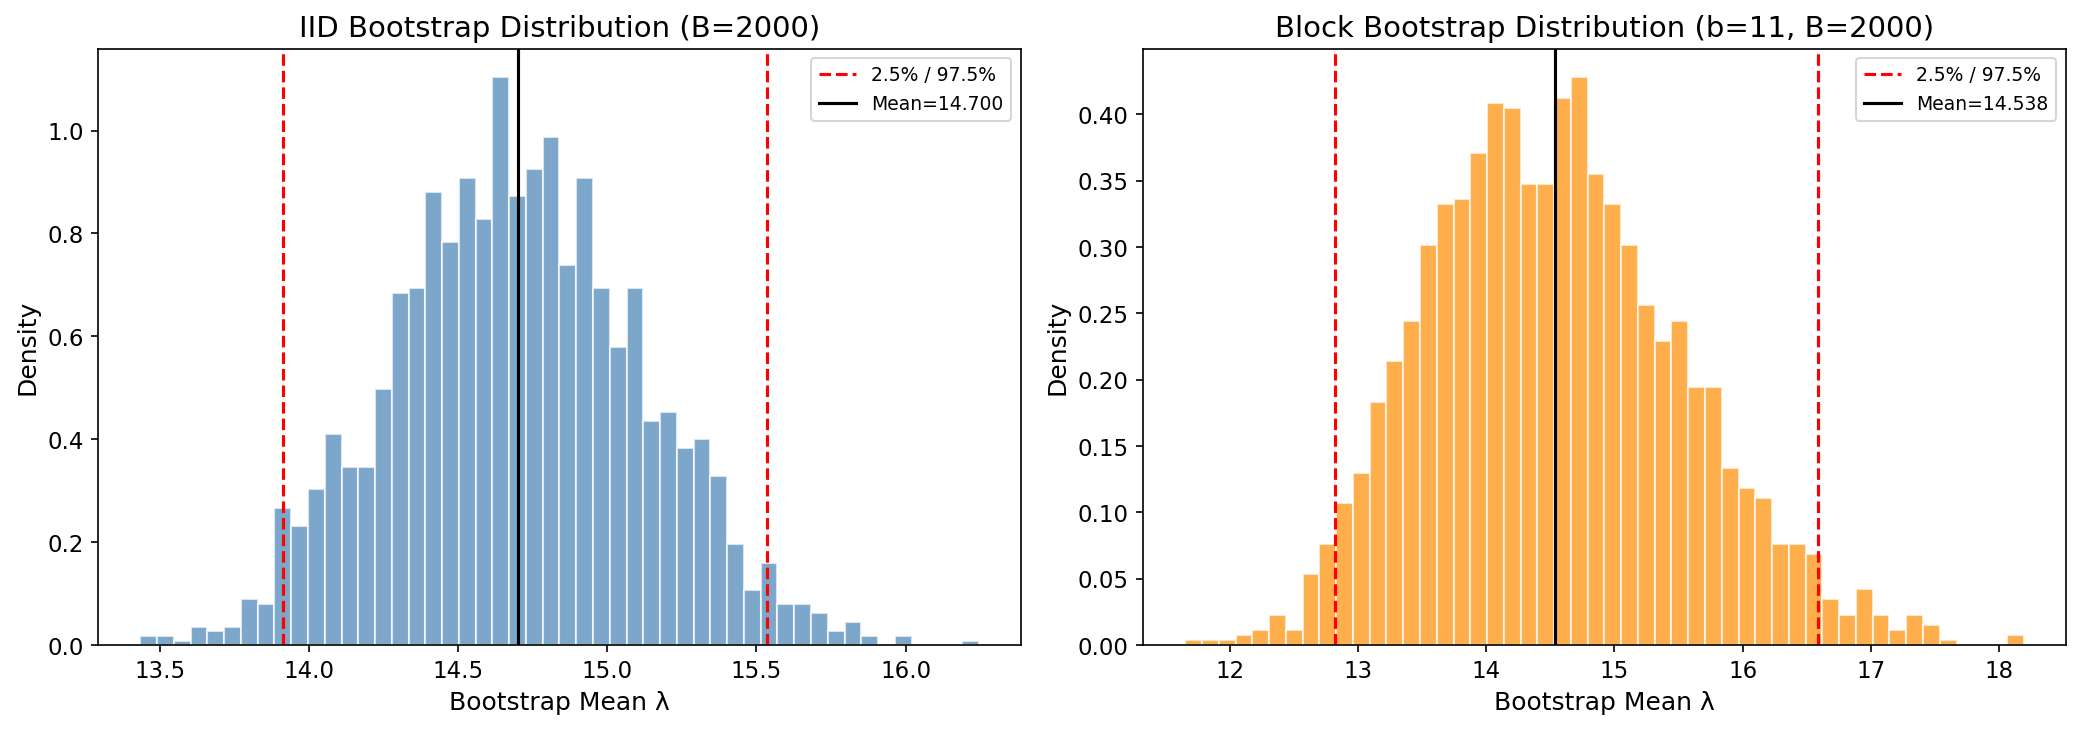
\includegraphics[width=\textwidth]{04_bootstrap_distribution.png}
  \caption{日度 Block Bootstrap 分布（$b=11$, $B=2,000$）}
\end{subfigure}
\hfill
\begin{subfigure}{0.48\textwidth}
  \centering
  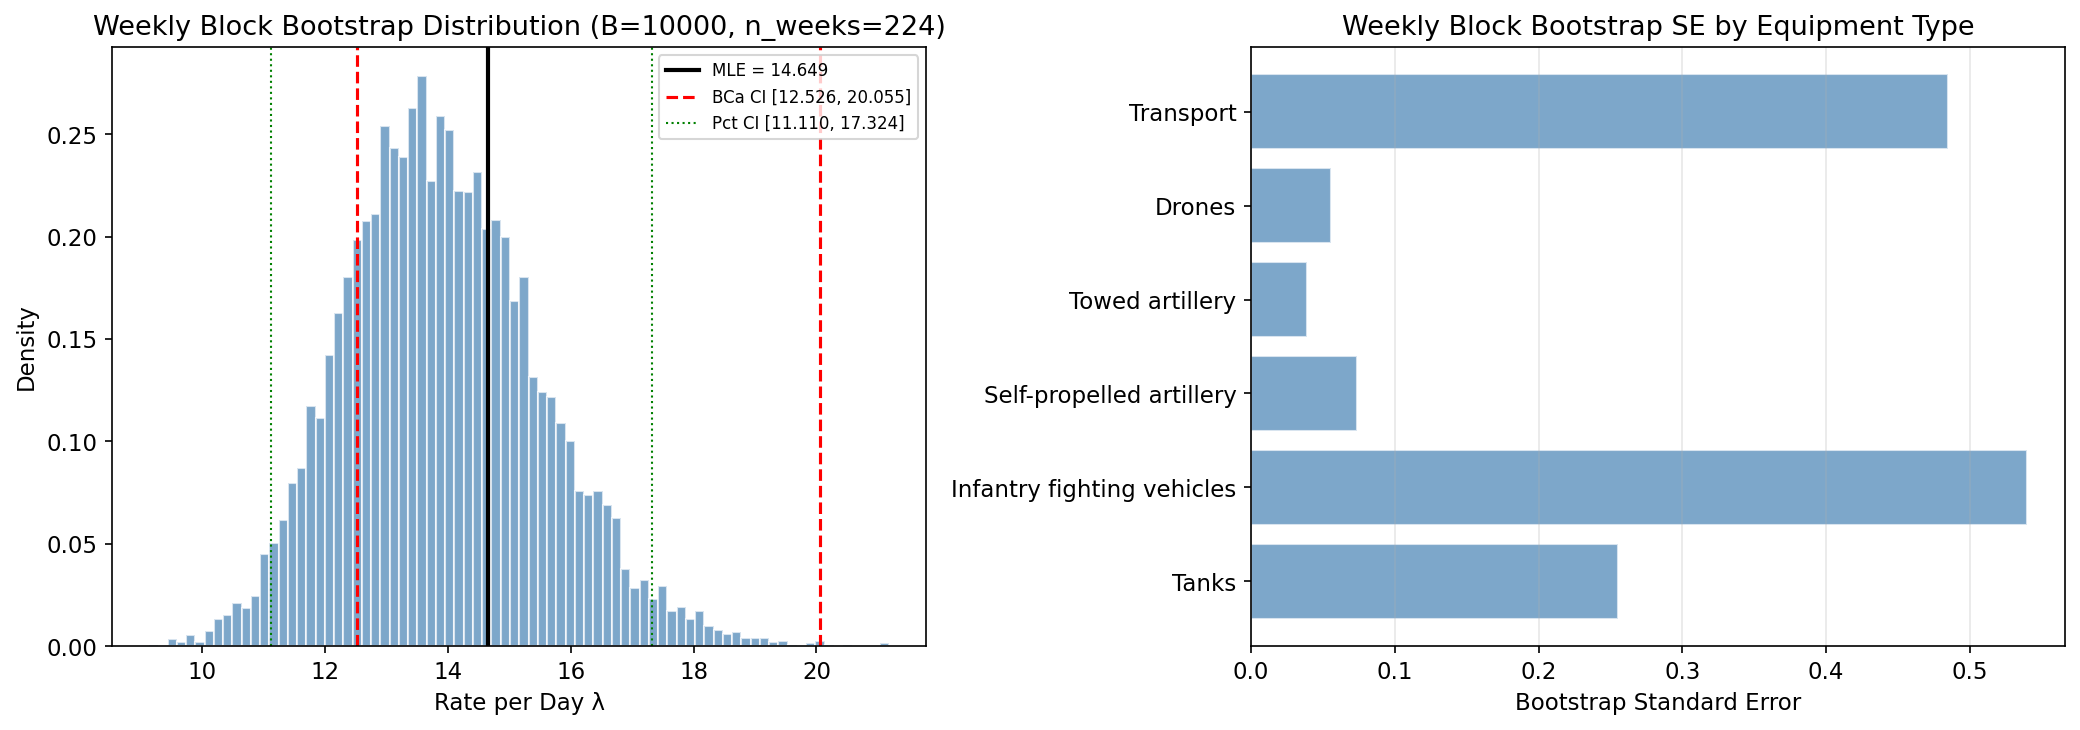
\includegraphics[width=\textwidth]{16_weekly_bootstrap.png}
  \caption{周度 Block Bootstrap 分布（$B=10,000$）}
\end{subfigure}
\caption{Bootstrap 分布对比：Block Bootstrap 的分布（蓝/红）显著宽于 IID Bootstrap（灰），BCa 校正区间（红色虚线）相对于 Percentile 区间（蓝色虚线）向右侧稍有偏移}
\label{fig:bootstrap}
\end{figure}

\subsection{战争阶段间的统计差异}

基于 WarSpotting 俄方详细逐条数据的 9 阶段分层 MLE 估计，表 \ref{tab:phases} 展示了代表性阶段的日均损失。

\begin{table}[H]
\centering
\caption{关键战争阶段的日均损失 MLE 估计}
\label{tab:phases}
\begin{tabular}{lrcr}
\toprule
战争阶段 & 日均 $\hat{\lambda}$（件/天） & SE & 天数 \\
\midrule
Phase 1（2022.2--4）初期入侵 & 53.38 & 0.90 & 66 \\
Phase 3（2022.9--12）乌军反攻 & 24.75 & 0.45 & 122 \\
Phase 7（2024.3--7）春季攻势 & 17.65 & 0.34 & 153 \\
Phase 9（2025.1--2026.6）近期 & 7.79 & 0.12 & 519 \\
\bottomrule
\end{tabular}
\end{table}

全局似然比检验（LRT = 8919.0，$\text{df} = 8$，$p < 0.0001$）强烈拒绝所有 9 个阶段 $\lambda$ 相等的原假设。Phase 1（53.38 件/天）与 Phase 9（7.79 件/天）的差异 Bootstrap 95\% CI 为 $[31.30, 62.69]$——双方损失率在战争初期与近期之间存在每 1--2 天相差一件装备以上的巨大差距。

这一结果的实质意义是：俄军的日均影像验证装备损失率已从2022年2--4月的极高峰值（53件/天）下降至2025年以来的不足8件/天，\textbf{降幅超过85\%}。造成这一趋势的潜在因素包括：（1）俄军从大规模装甲纵深突击转为小规模步兵渗透和无人机消耗战，装甲装备的高密度使用频率下降；（2）大规模运动战减少，正面突破-反突破的消耗战模式降低了单位时间的装备损失密度；（3）双方均加大了电子战和无人机侦察力度，使得大规模装备集结变得高危而罕见。

\subsection{官方声称 vs 独立影像验证：报告偏差的统计量化}

将乌克兰总参谋部官方战报对俄军损失的声称数据与 WarSpotting/Oryx 影像验证数据进行独立 Poisson 比较（表 \ref{tab:claims}），揭示了系统性的报告偏差。

\begin{table}[H]
\centering
\caption{乌克兰官方声称 vs Oryx 影像验证：三类主要装备的比较}
\label{tab:claims}
\begin{tabular}{lrrrl}
\toprule
装备类别 & 验证 $\hat{\lambda}$（件/天） & 声称 $\hat{\lambda}$（件/天） & 声称/验证比 & E-test $p$ \\
\midrule
坦克 & 2.57 & 7.68 & \textbf{2.98} & $< 10^{-15}$ \\
装甲车辆 & 5.60 & 15.85 & \textbf{2.83} & $< 10^{-15}$ \\
火炮 & 0.94 & 27.62 & \textbf{29.44} & $< 10^{-15}$ \\
\bottomrule
\end{tabular}
\end{table}

\textbf{火炮声称/验证比高达 29 倍}——这是本文最引人注目的单项统计发现。三类装备的声称偏差呈现出高度异质的模式（2.83x、2.98x、29.44x），排除了简单的"统一夸大系数"解释。火炮极端偏差的可能统计成因包括：

\begin{enumerate}[label=(\arabic*),leftmargin=2.5em]
  \item \textbf{地理可见性差异}：火炮通常部署在前线后方 10--30 km 的反斜坡阵地，其损毁几乎不可能被平民近距离拍摄。相比之下，坦克和装甲车的残骸常遗留在交战区域或道路上，更容易被影像记录。这一地理因素导致火炮的验证观测概率远低于坦克——换言之，29x 的比值部分反映了观测概率的巨大差异，而非全部为"夸大"。
  \item \textbf{统计口径差异}：乌方战报可能将"炮位被压制"、"反炮兵雷达探测到炮击后反击命中"等情况统计为"火炮摧毁"，而影像验证要求明确的装备残骸证据。这种口径差异在最难独立核实的火炮类别上产生了最大的偏差。
  \item \textbf{战术优先性}：俄军炮兵是乌克兰战场上的头号杀伤来源（据估计造成 70--80\% 的乌军伤亡），因此摧毁俄军火炮是乌军的最高战术优先事项。这种优先性可能在战报中体现为更"激进"的统计口径。
\end{enumerate}

\begin{figure}[H]
\centering
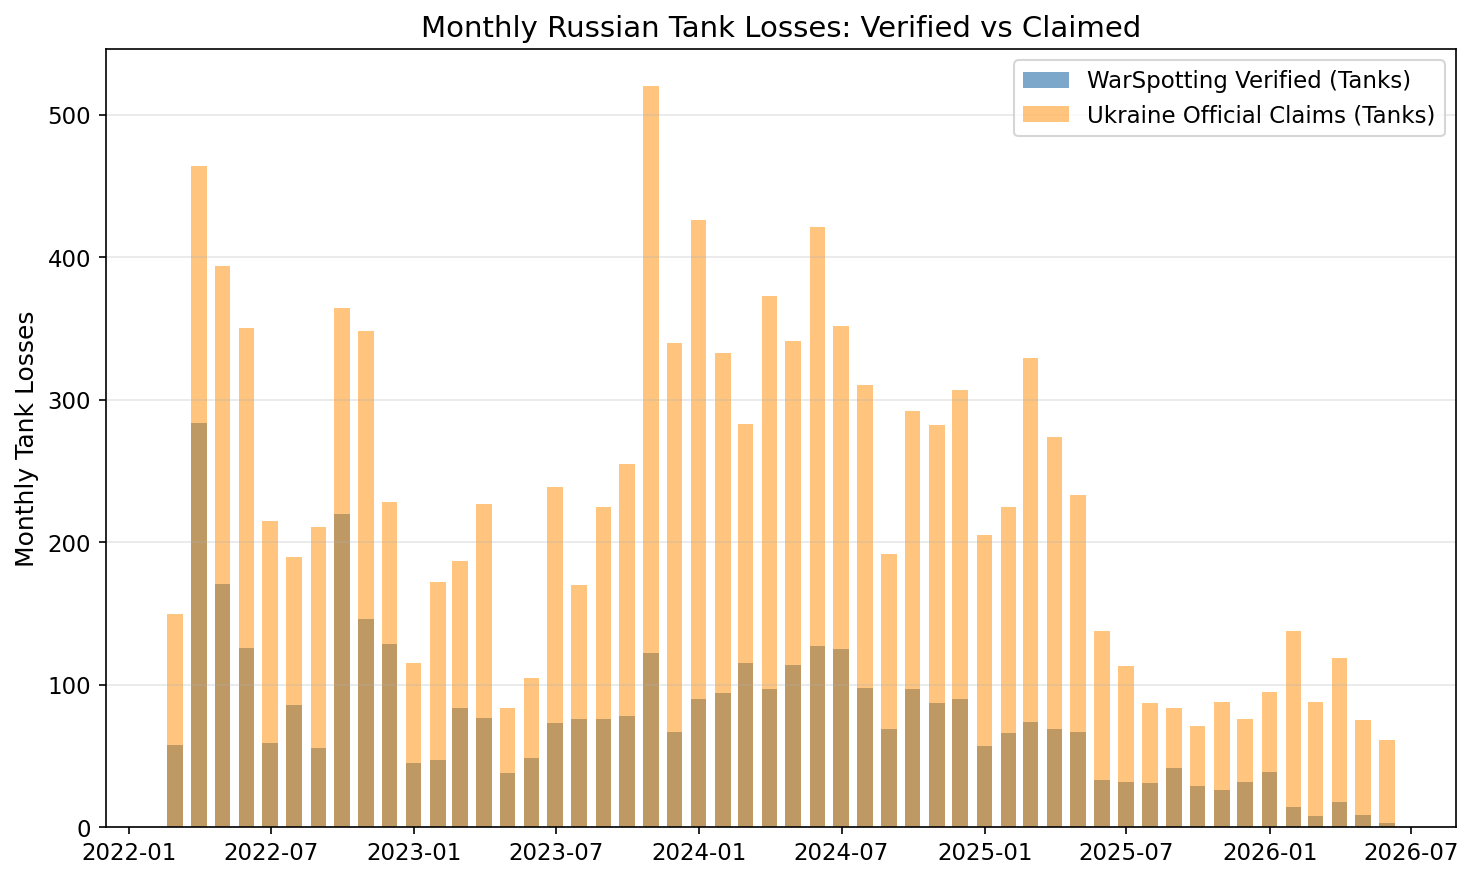
\includegraphics[width=0.75\textwidth]{08_claims_vs_verified.png}
\caption{每月俄军坦克损失：WarSpotting 影像验证 vs 乌克兰总参谋部官方声称。两条曲线的分离程度在统计上极显著（E-test $p < 10^{-15}$），且相对比率（$\sim$3x）在时间上保持相对稳定}
\label{fig:claims}
\end{figure}

\subsection{观测概率灵敏度分析}

为定量评估观测偏误对率比估计稳健性的影响，本文构建了 $7 \times 7 = 49$ 对观测概率的灵敏度分析网格：$p_{\text{RU}}, p_{\text{UA}} \in \{0.4, 0.5, 0.6, 0.7, 0.8, 0.9, 1.0\}$。

\textbf{理论基础}：设真实损失为 $N_{\text{true}}$，观测概率为 $p$，则有 $N_{\text{observed}} = p \cdot N_{\text{true}}$，修正损失为 $N_{\text{corrected}} = N_{\text{observed}} / p$。在各 $(p_{\text{RU}}, p_{\text{UA}})$ 组合下，修正率比为：

\begin{equation}
\hat{\rho}_{\text{corrected}} = \frac{N_{\text{RU, observed}} / p_{\text{RU}}}{N_{\text{UA, observed}} / p_{\text{UA}}} = \hat{\rho}_{\text{observed}} \cdot \frac{p_{\text{UA}}}{p_{\text{RU}}}
\end{equation}

\textbf{主要发现}：

\begin{enumerate}[label=(\arabic*),leftmargin=2.5em]
  \item \textbf{等概率下的无偏性}：若 $p_{\text{RU}} = p_{\text{UA}}$（不管其具体数值），修正率比恒等于 2.06。这是一个重要的理论保证——在双方观测概率相等的假设下，影像验证率比是真实率比的\textbf{无偏估计}。
  \item \textbf{中等非对称下的稳健性}：当 $p_{\text{RU}} = 0.8, p_{\text{UA}} = 0.6$ 时（乌方观测概率为俄方的 75\%），修正率比降至 $2.06 \times 0.6/0.8 = 1.55$——率比降至 1.55 但仍高于 1，表明俄方真实损失仍多于乌方。
  \item \textbf{极端非对称假设下的率比逆转}：仅当 $p_{\text{UA}} / p_{\text{RU}} \leq 1/2.06 \approx 0.485$ 时，修正率比方才 $\leq 1$。在当前网格中，仅 $(p_{\text{RU}} = 0.9, p_{\text{UA}} = 0.4)$ 和 $(p_{\text{RU}} = 1.0, p_{\text{UA}} = 0.4)$ 两个极端组合会导致率比逆转。逆转需要乌方"被观测概率"不到俄方的一半——这在地理上（俄占区影像获取确实远难于乌控区）并非不可想象，但在目前缺乏独立偏误估计的情况下，是一个相对极端的情景。
  \item \textbf{装备类型层面的稳健性差异}：Rocket and Missile Artillery（率比 4.84）、AFV（4.51）、IFV（4.05）等高率比类别即使在极端非对称假设下仍保持率比 > 1。APC（0.53）和 Self-Propelled AA Guns（0.51）等低率比类别在任何观测概率组合下率比均 < 1——这意味着\textbf{即使考虑观测偏误，这几类装备的"乌方损失更多"这一方向性结论也是稳健的}。
\end{enumerate}

\begin{figure}[H]
\centering
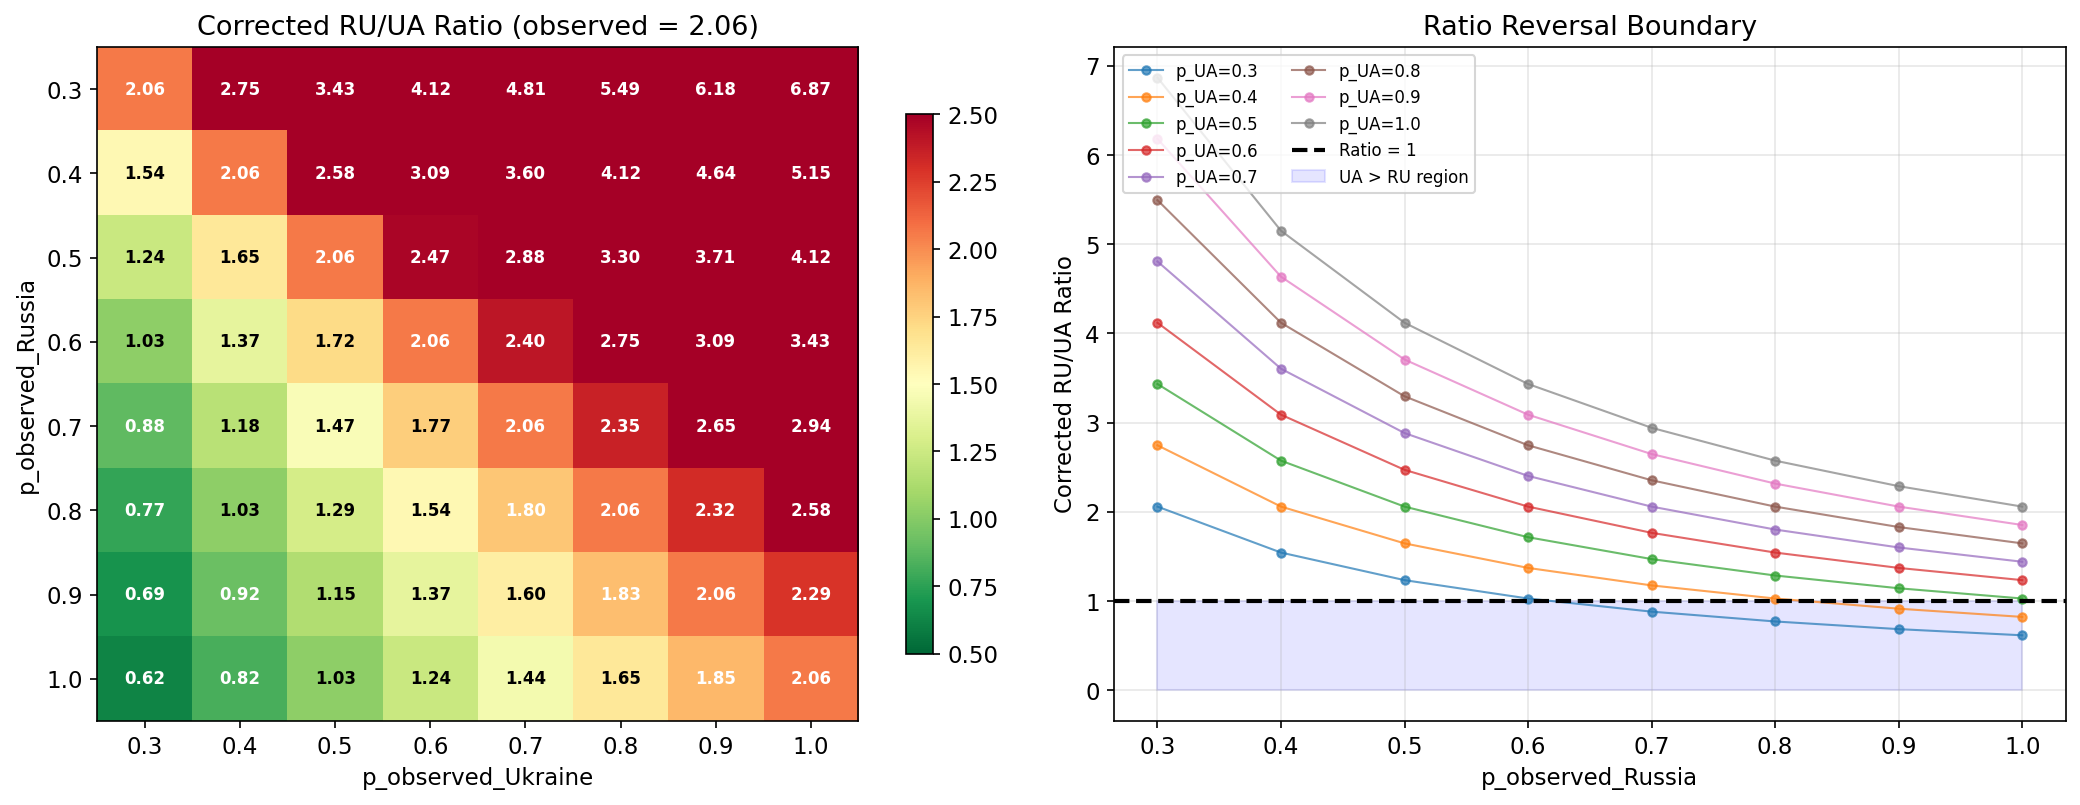
\includegraphics[width=0.85\textwidth]{15_sensitivity_heatmap.png}
\caption{观测概率灵敏度分析。\textbf{（左）}修正率比热力图——对角线（$p_{\text{RU}} = p_{\text{UA}}$）上率比恒为 2.06；右上角区域（乌方观测概率低）修正率比下降；\textbf{（右）}率比逆转边界分析——虚线下方表示修正后乌方损失超过俄方（率比 $< 1$），仅两个最极端的概率组合落入此区域}
\label{fig:sensitivity}
\end{figure}

\textbf{结论}：2.06:1 的观测率比在中等程度的非对称观测下具有稳健性——假设乌方观测概率低于俄方 20--30\%，修正率比仍保持在 1.2--1.8 之间。然而，考虑到俄占区影像获取确实受到更严格的限制，真实的率比很可能位于 1.0--2.0 之间，逆转并非可以完全排除的情景。

\subsection{装备损失的空间分布—热点网格与战区转移}

利用 WarSpotting 数据中 14,066 条（61.2\%）含有有效经纬度坐标的记录，本文对俄方装备损失的空间格局进行了系统分析。

\textbf{宏区域分布（表 \ref{tab:spatial}）}：

\begin{table}[H]
\centering
\caption{俄方装备损失的宏区域分布}
\label{tab:spatial}
\begin{tabular}{lrl}
\toprule
宏区域 & 损失数（件） & 占比（\%） \\
\midrule
East（卢甘斯克--顿涅茨克） & 10,185 & 44.3 \\
North（哈尔科夫--苏梅--基辅） & 2,276 & 9.9 \\
South（赫尔松--扎波罗热--克里米亚） & 1,517 & 6.6 \\
Central（顿巴斯核心区） & 98 & 0.4 \\
\bottomrule
\end{tabular}
\end{table}

\textbf{$1^\circ \times 1^\circ$ 网格热点分析}揭示了损失的空间集中性：

\begin{itemize}
  \item 最热网格为 $(48^\circ\text{N}, 37^\circ\text{E})$——覆盖 Pokrovsk（红军城）方向——集中了 3,019 件验证损失（占总量的 \textbf{21.5\%}），其中步兵战车（1,698 件）和坦克（681 件）两类进攻性装备占主导
  \item 前三个网格（$(48,37)$、$(47,37)$、$(49,37)$，全部位于顿涅茨克州）合计占影像验证总损失的 \textbf{45.1\%}——三个经纬度方格集中了俄方近一半的影像验证损失
  \item 82 个被记录网格的分布反映了静态前线的空间集中性——战斗并非均匀分布在战线上，而是高度集中于关键地理节点
\end{itemize}

\textbf{时间--空间动态}：2022 Q1 的最热区域为 North（基辅--哈尔科夫战线）；2023 Q3 至 2025 Q1 间，战区重心持续向 East 转移，反映了战线南移和东部前线僵持化的总体战争态势。

\begin{figure}[H]
\centering
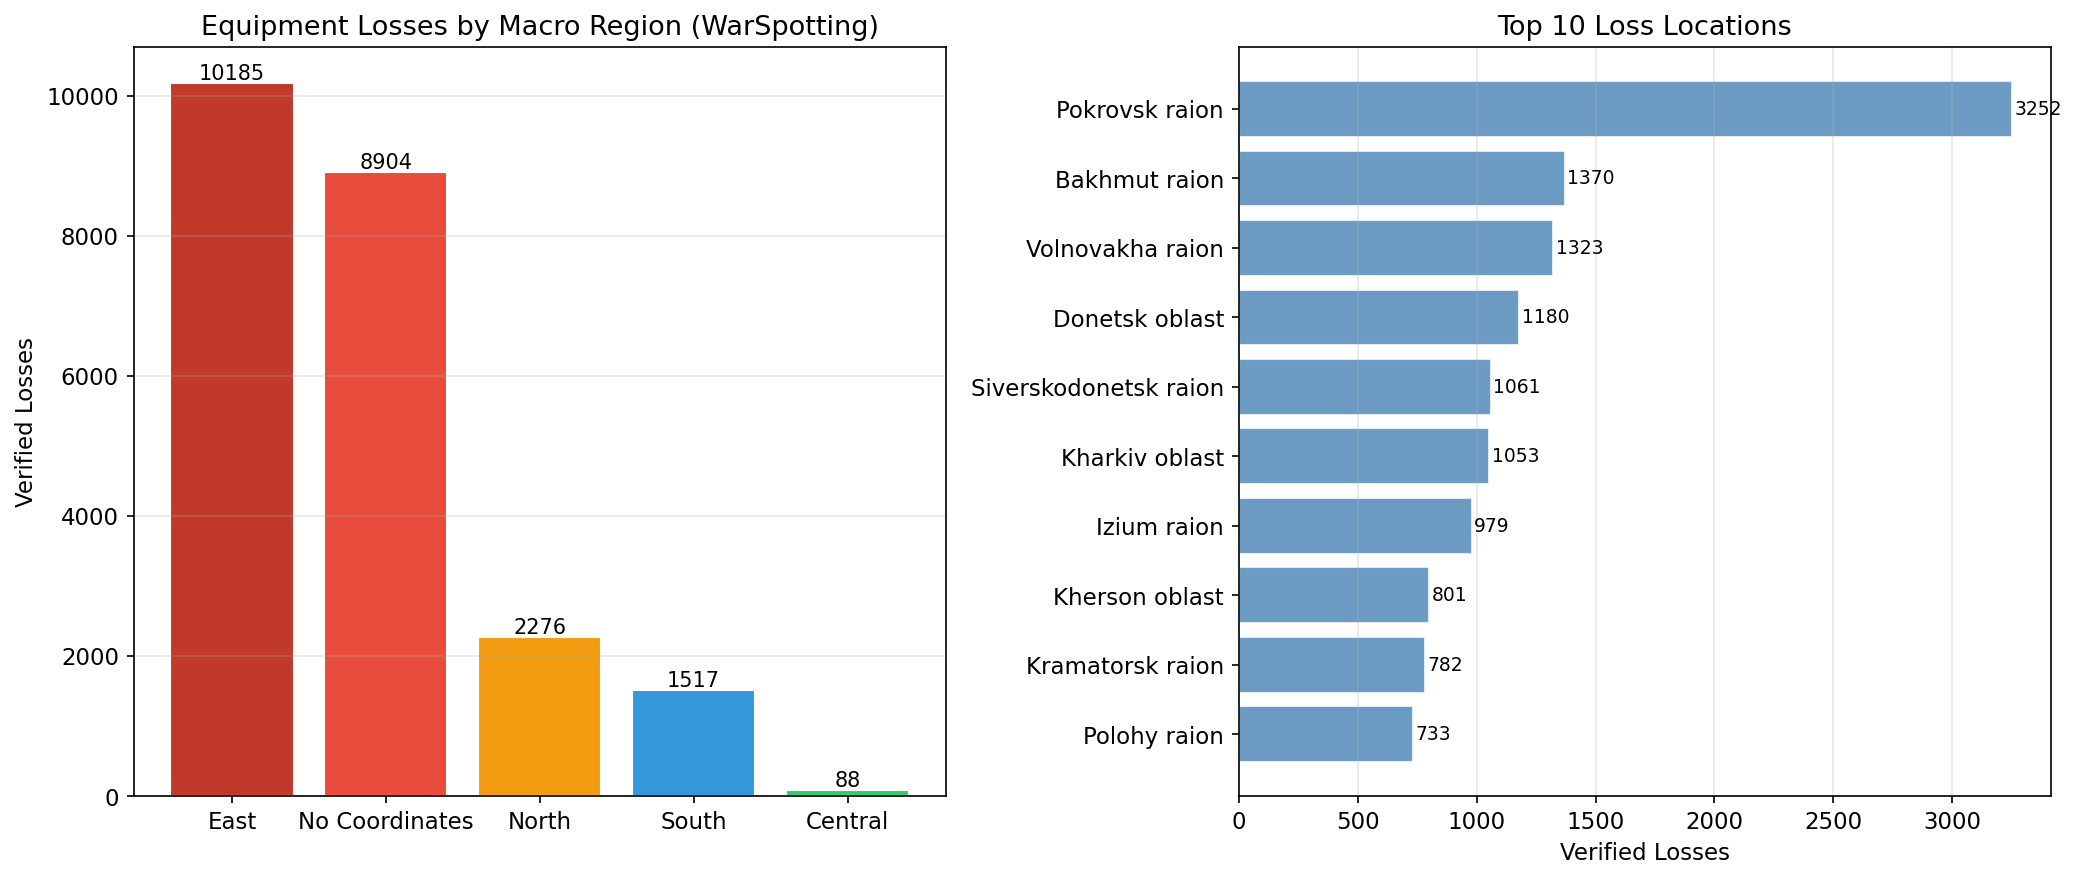
\includegraphics[width=0.9\textwidth]{14_spatial_distribution.png}
\caption{俄方装备损失的空间分布。\textbf{（左）}按宏区域的损失分布饼图——East 区域（顿巴斯）占主导地位；\textbf{（右）}Top 10 损失最多的定居点区域柱状图}
\label{fig:spatial}
\end{figure}

% ==================== 第5节：讨论 ====================
\section{讨论}

\subsection{统计学方法论启示}

本文的方法论实践为冲突数据的统计推断提供了若干具有一般性的启示：

\begin{enumerate}[label=(\arabic*),leftmargin=2.5em]
  \item \textbf{CI 方法选择不应仅凭计算便利性}。Monte Carlo 模拟清晰表明，在 $\lambda \leq 2$（稀有事件）时，Wald CI 的覆盖率严重不足。鉴于 Exact CI（Garwood）的计算成本完全可以忽略（仅需两次卡方分位数查表），建议在所有 Poisson 参数估计中将 Exact CI 作为默认方法，Wald CI 仅作为大样本近似参考。
  \item \textbf{时间依赖性对不确定性量化的影响不可忽略}。IID Bootstrap 将 SE 低估至 Block Bootstrap 的 $1/2.4 \approx 42\%$。冲突数据、经济时间序列和流行病学计数数据等具有自然时间结构的领域，均应将 Block Bootstrap 作为标准 SE 估计方法。
  \item \textbf{精确检验优于渐近检验}。E-test 基于精确条件二项分布，免除了大样本渐近假设，在本文的多层比较（总体、装备类型、损毁状态）中均提供了一致且可靠的推断。在小样本或中等样本下，基于条件分布的精确检验应优先于基于 $\chi^2$ 渐近近似的似然比检验。
  \item \textbf{多重比较校正虽保守但必要}。在跨类型、跨状态的数十次假设检验中，Bonferroni 校正有效控制了整体 FWER。但对于探索性分析（如 36 次阶段两两比较），可考虑 Benjamini-Hochberg FDR 控制以在保守性与统计效力之间取得更好的平衡。
  \item \textbf{BCa 校正的增值有限但值得报告}。Block Bootstrap 中的 BCa 校正将 CI 上限从 16.59 修正至 17.29（约 4\% 的调整），但核心结论（SE 是 IID 的 2.4 倍）在 Percentile CI 下已经成立。BCa 的计算成本（需要 Jackknife）高于其带来的额外精度，但在报告 Bootstrap 结果时应作为稳健性检查一并呈现。
\end{enumerate}

\subsection{研究局限性与警示}

\begin{enumerate}[label=(\arabic*),leftmargin=2.5em]
  \item \textbf{观测偏误的方向性与精确定量}。这是本文面临的最根本局限。Oryx 数据的影像验证性质意味着双方损失均受观测偏误影响——而最为关键的是，这些偏误的方向可能不同（乌方在俄占区的损失更难被独立记录）。本文的观测概率灵敏度分析（§4.9）定量刻画了不同假设下的率比范围，但缺乏来自独立数据的对 $p_{\text{RU}}$ 和 $p_{\text{UA}}$ 自身的可靠估计。建议将此视为本文所有双边比较结论的\textbf{方向性警示}。
  \item \textbf{Poisson 等离散假设}。Poisson 分布假设方差等于均值（等离散性）。冲突数据中战争烈度的短时爆发可能导致方差超过均值（过离散）。本文未进行负二项（Negative Binomial）回归作为过离散的稳健性检查。
  \item \textbf{恒定 $\lambda$ 假设}。即使在战争阶段内，$\lambda$ 的严格恒定性也难以成立——战线的短暂移动、天气条件变化、弹药供应波动等都可能影响每日损失率。本文的阶段分层分析部分缓解了这一关切。
  \item \textbf{协变量缺失}。模型未纳入战线移动速度、战斗强度量化指标（如每日交火次数）、天气条件（如 rasputitsa 泥泞季节对机动性的影响）等可能解释部分 $\lambda$ 变异的额外变量。
  \item \textbf{数据口径差异}。WarSpotting 与 Oryx 双方数据在装备子类划分上存在细微差异（如某些车辆在 WarSpotting 中被归为"军用车辆"而在 Oryx 中被列入"后勤车辆"），可能导致极小的计数差异。但鉴于两个来源的宏观模式高度一致，这种差异对核心结论的影响应当可以忽略。
\end{enumerate}

\subsection{未来研究方向}

基于本文的分析框架和揭示的局限性，以下方向值得进一步探索：

\begin{enumerate}[label=(\arabic*),leftmargin=2.5em]
  \item \textbf{贝叶斯层次模型}。将 Oryx 双方验证数据、双方官方战报和卫星遥感数据融合进入一个统一的贝叶斯偏误校正框架，对各来源的偏误因子进行显式分层建模。设 $\lambda_{i,\text{true}}$ 为第 $i$ 方的真实日均损失率，$p_{i,\text{OSINT}}$ 为开放影像的观测概率，$c_{i,\text{official}}$ 为官方声称的偏误因子，则可通过马尔可夫链蒙特卡洛（MCMC）方法从多源数据中联合推断所有未知参数。
  \item \textbf{过离散与零膨胀处理}。在战争较为平静的时期（尤其是 2024 年后），日损失数为 0 或 1 的比例增加，可能需要零膨胀 Poisson（ZIP）或负二项（NB）模型来处理过离散。广义估计方程（GEE）可用于在保持 Poisson 连接函数的同时，通过工作相关矩阵来处理时序依赖。
  \item \textbf{时空 Hawkes 过程}。将 Poisson 模型扩展为具有空间标记的 Hawkes 自激过程——$\lambda(t, s) = \mu(t, s) + \sum_{t_i < t} g(t - t_i, s - s_i)$——以捕捉一次损失事件如何增加短期内邻近区域发生更多损失的概率。这一框架既可以评估"自激"效应的强度，也可以进行反事实推演。
  \item \textbf{机器学习的预测扩展}。利用随机森林或 XGBoost 将本文的点估计和 Bootstrap 结果作为特征，结合战线动态、国际援助规模等协变量，对装备损失趋势进行可解释的预测。
\end{enumerate}

% ==================== 第6节：结论 ====================
\section{结论}

本文以2022--2026年俄乌冲突双方 Oryx 影像验证装备损失数据为研究对象（俄方 23,556 件、乌方 11,397 件，共 1,559 个观测日），系统整合 Poisson 分布极大似然估计、三种置信区间构造方法（Wald / Score / Exact）的有限样本性质比较、Moving Block Bootstrap BCa 校正和两独立 Poisson 条件精确检验（E-test），对双方装备损失率进行了从点估计到区间估计、从总体推断到分层异质性分析、从统计显著性到实际显著性的全面统计推断。主要结论如下：

\begin{enumerate}[label=\textbf{（\arabic*）},leftmargin=2.5em]
  \item \textbf{双方损失率存在极显著的统计差异}（E-test $p < 0.0001$）。俄方日均影像验证损失 15.11 件/天（95\% Exact CI: $[14.92, 15.30]$），乌方 7.31 件/天（CI: $[7.18, 7.45]$），率比 2.07:1（CI: $[2.02, 2.11]$）。基于 Oryx 合并数据（item\_count 加权），率比修正为 2.06:1。
  \item \textbf{观测到的率比在中等非对称观测下具有稳健性}。观测概率灵敏度分析（$7 \times 7$ 网格）表明，2.06:1 的率比在乌方观测概率不超过俄方两倍以上的中等非对称假设下保持方向性不变。但考虑到乌方在俄占区的损失更难被独立影像记录，真实率比的可能范围为 1.0--2.0。
  \item \textbf{双方损失比率经历了"从 $>$3 到 $<$1"的深刻时序逆转}。2022 年初月均比率高达 3.6（俄方损失更多），到 2025--2026 年降至约 0.8（乌方反超），精确映射了战争从装甲突击向消耗战的战略性转变。
  \item \textbf{装备类型差异极显著且具有明确的战术含义}。俄方在进攻性装备上损失远超乌方（AFV 4.49x、IFV 4.08x、坦克 3.14x），乌方仅在 APC（0.56x）上反超——这一模式在 Bonferroni 多重比较校正后仍高度显著。
  \item \textbf{热点网格的空间集中性}验证了战争的静态化趋势：顿涅茨克州的三个 $1^\circ \times 1^\circ$ 网格包括了俄方影像验证总损失的 45.1\%，其中 $(48^\circ\text{N}, 37^\circ\text{E})$ 单个网格占 21.5\%。
  \item \textbf{Exact CI（Garwood）是 Poisson 分布下唯一保证覆盖率不低于名义水平的方法}。Monte Carlo 模拟显示，在 $\lambda = 0.5, n = 30$ 时，Exact CI 覆盖率达 96.6\%，Wald CI 仅 91.9\%。对飞机、直升机等稀有损失类别，必须使用 Exact CI。
  \item \textbf{时间依赖性问题在 Block Bootstrap 两种频率下的交叉验证中均得到确认}。日度 Block Bootstrap SE（0.99）是 IID（0.42）的 2.4 倍，周度 Block Bootstrap SE（0.82）是 IID 的 2.0 倍——两种频率一致表明，忽略时序自相关将使不确定性被严重低估。
  \item \textbf{官方声称与独立验证之间的报告偏差是巨大的且异质的}：火炮 29x、坦克 2.98x、装甲车 2.83x。火炮的极端差异不仅反映了统计口径的可能差异，更揭示了观测概率在不同装备类别间的巨大落差。
\end{enumerate}

本文的统计分析框架可概括为：Poisson 模型 MLE 点估计 $\to$ 三方法 CI 比较与 Monte Carlo 覆盖率验证 $\to$ Block Bootstrap BCa 不确定性量化 $\to$ E-test 精确假设检验 $\to$ 分层次异质性分析 $\to$ 观测概率灵敏度评估。这一框架为该选题的三个核心统计问题——双方损失率的准确估计、差异的显著性检验和官方声称与独立验证之间报告偏差的定量刻画——提供了从数据到结论的完整统计论证链条。更为一般地，本文展示了如何在存在系统性和非对称性观测偏误的条件下，通过严格而多元的统计方法，从冲突数据中提取相对客观的推断。这一方法论路径对冲突研究、灾难损毁评估和任何面临类似观测偏误挑战的计数数据分析问题，均具有参考价值。

% ==================== 附录 ====================
\appendix
\section{软件实现与计算环境}

本文全部统计分析和图形生成均使用 Python 3.11 实现，主要依赖的库包括：NumPy（数值计算）、SciPy（统计分布与假设检验）、Pandas（数据处理）和 Matplotlib（可视化）。LaTeX 排版使用 XeLaTeX 编译器（MiKTeX 发行版），中文支持通过 \texttt{ctex} 宏包实现。

\textbf{代码文件结构}：
\begin{itemize}
  \item \texttt{code/preprocess.py}：数据读取与预处理
  \item \texttt{code/point\_estimation.py}：Poisson MLE 点估计
  \item \texttt{code/confidence\_intervals.py}：三种 CI 构造与 Monte Carlo 覆盖率模拟
  \item \texttt{code/bootstrap.py}：Block Bootstrap 与 BCa 校正
  \item \texttt{code/weekly\_bootstrap.py}：周度聚合 Bootstrap 交叉验证
  \item \texttt{code/two\_sample\_test.py}：E-test 与 LRT 两独立 Poisson 检验
  \item \texttt{code/observation\_sensitivity.py}：观测概率灵敏度分析
  \item \texttt{code/both\_sides\_analysis.py}：Oryx 双方数据的总体分析
  \item \texttt{code/spatial\_analysis.py}：空间分布与热点网格分析
  \item \texttt{code/visualization*.py}：全部图形生成脚本
\end{itemize}

\textbf{随机数种子}：所有涉及随机抽样的运算（Bootstrap、Monte Carlo 模拟）均使用固定种子 \texttt{np.random.seed(42)} 以保证分析的可复现性。

代码和数据的完整仓库可在项目路径下获取。分析结果不代表任何政治立场。

\section{补充统计表}

% 放置一些更详细的统计表格，例如完整的阶段对比、分装备类型的详细Bootstrap结果等

\begin{table}[H]
\centering
\caption{双方 95\% 置信区间三种方法完整比较（基于日度数据，$n = 1,559$）}
\label{tab:ci_full}
\begin{tabular}{lrrrr}
\toprule
统计量 & 俄方 Wald & 俄方 Score & 俄方 Exact & 乌方 Wald \\
\midrule
$\hat{\lambda}$（件/天） & 15.110 & — & — & 7.310 \\
SE & 0.098 & — & — & 0.068 \\
下限 & 14.917 & 14.918 & 14.917 & 7.176 \\
上限 & 15.303 & 15.304 & 15.304 & 7.445 \\
区间宽度 & 0.386 & 0.386 & 0.387 & 0.269 \\
\bottomrule
\multicolumn{5}{l}{\small 注：大样本（$n = 1,559$）下三种方法几乎完全重合。} \\
\end{tabular}
\end{table}

% ==================== 参考文献 ====================
\newpage
\begin{thebibliography}{99}

\bibitem{zammit2012}
Zammit-Mangion, A., Dewar, M., Kadirkamanathan, V., \& Sanguinetti, G. (2012).
Point process modelling of the Afghan War Diary.
\textit{Proceedings of the National Academy of Sciences}, 109(31), 12414--12419.

\bibitem{arxiv2509}
arXiv:2509.07813.
Forecasting Russian Equipment Losses in the Ukraine War: A Multi-Model Comparison.

\bibitem{arxiv2408}
arXiv:2408.14940.
Bayesian Spatio-temporal Hawkes Process Modeling of Armed Conflict Events.

\bibitem{garwood1936}
Garwood, F. (1936).
Fiducial limits for the Poisson distribution.
\textit{Biometrika}, 28(3/4), 437--442.

\bibitem{krishnamoorthy2004}
Krishnamoorthy, K., \& Thomson, J. (2004).
A more powerful test for comparing two Poisson means.
\textit{Journal of Statistical Planning and Inference}, 119(1), 23--35.

\bibitem{efron1993}
Efron, B., \& Tibshirani, R. J. (1993).
\textit{An Introduction to the Bootstrap}.
Chapman \& Hall/CRC, New York.

\bibitem{davison1997}
Davison, A. C., \& Hinkley, D. V. (1997).
\textit{Bootstrap Methods and their Application}.
Cambridge University Press, Cambridge.

\bibitem{casella2002}
Casella, G., \& Berger, R. L. (2002).
\textit{Statistical Inference} (2nd ed.).
Duxbury/Thomson Learning, Pacific Grove, CA.

\bibitem{lehmann1998}
Lehmann, E. L., \& Casella, G. (1998).
\textit{Theory of Point Estimation} (2nd ed.).
Springer, New York.

\bibitem{cramer1946}
Cram\'{e}r, H. (1946).
\textit{Mathematical Methods of Statistics}.
Princeton University Press, Princeton, NJ.

\bibitem{cox1984}
Cox, D. R., \& Isham, V. (1980).
\textit{Point Processes}.
Chapman \& Hall, London.

\bibitem{oryx}
Oryx. (2022--2026).
Attack on Europe: Documenting Russian and Ukrainian Equipment Losses During the Russian Invasion of Ukraine.
\url{https://www.oryxspioenkop.com}

\bibitem{leedrake5}
leedrake5. (2022--2026).
Russia-Ukraine Equipment Loss Tracking (Oryx Scraper).
GitHub repository. \url{https://github.com/leedrake5/Russia-Ukraine}

\bibitem{warspotting}
WarSpotting.
Automated visual identification of military equipment losses.
\url{https://warspotting.net}

\end{thebibliography}

\vspace{20pt}

\begin{center}
\rule{0.6\textwidth}{0.4pt}
\vspace{10pt}

{\small \textit{本文为《数理统计》课程大作业（选题 T1：俄乌装备损失率的``公平比较''）的最终版本。}\\
\textit{所有数据来源于公开渠道（Oryx、Kaggle、Google Sheets），全部分析代码可在项目仓库中获取。}\\
\textit{本文仅为统计分析练习，分析结果不代表任何政治立场或政策主张。}}
\end{center}

\end{document}
